%%%% using 'arara' 4.0
% arara: xelatex: {synctex: yes, interaction: nonstopmode}
% arara: bibtex
% arara: xelatex: {synctex: yes, interaction: nonstopmode}
% arara: xelatex: {synctex: yes, interaction: nonstopmode}

% arara: indent: {overwrite: yes}

% arara: clean: { extensions: [aux, bcf, cod, blg, lof, lot, out, toc, log, xml, bak0 ] }

\documentclass[review]{elsarticle}

% Figures Links, mittig und rechts platzieren
\usepackage[export]{adjustbox}
\usepackage{caption}
\usepackage{subcaption}

\graphicspath{{../../../../04_figures/02_results/}{./}{../../../../04_figures/01_data/}} 

% prevents that appendices are moved behind references
\usepackage{placeins}

\usepackage[nolist]{acronym}

\usepackage{longtable}
\usepackage{booktabs}
\usepackage{multirow}
\usepackage{float} 

% https://tex.stackexchange.com/questions/223149/warning-text-page-x-contains-only-floats-how-to-suppress-this-warning
\usepackage{silence}
\WarningFilter{latex}{Text page}

% https://tex.stackexchange.com/questions/165115/getting-not-defining-perthousnad-and-not-defining-micro-when-compiling-beamer
\usepackage{textcomp}

% enable subsubsection as 4th level https://tex.stackexchange.com/questions/60209/how-to-add-an-extra-level-of-sections-with-headings-below-subsubsection
\usepackage{titlesec}
\setcounter{secnumdepth}{4}
\titleformat{\subsubsection}
{\normalfont\small\bfseries}{\thesubsubsection}{1em}{}
\titlespacing*{\subsubsection}
{0pt}{3.25ex plus 1ex minus .2ex}{1.5ex plus .2ex}

\titleformat{\subsection}
{\normalfont\small\bfseries}{\thesubsection}{1em}{}
\titlespacing*{\subsection}
{0pt}{3.25ex plus 1ex minus .2ex}{1.5ex plus .2ex}

% enable linking to subsubsection
\setcounter{secnumdepth}{3}

% various symbols, e.g. \degree
\usepackage{gensymb}

\usepackage[hidelinks]{hyperref}

\usepackage{lineno}
\modulolinenumbers[5]

% set autoref abbr for appendix
\newcommand*{\Appendixautorefname}{appendix}

\journal{Ecological Modelling}

% line breaks in table cells
\newcommand{\specialcell}[2][l]{%
  \begin{tabular}[#1]{@{}l@{}}#2\end{tabular}}

% tilde
\newcommand{\mytilde}{\raise.17ex\hbox{$\scriptstyle\mathtt{\sim}$}}

%% APA style
\bibliographystyle{model5-names}\biboptions{authoryear}

\begin{document} 

\begin{frontmatter}

	\title{Analyzing the importance of spatial autocorrelation in hyperparameter tuning and performance estimation of machine-learning algorithms for spatial data.} 

	%% Group authors per affiliation:
	\author[FSU]{Patrick Schratz}
	\cortext[mycorrespondingauthor]{Corresponding author}
	\ead{patrick.schratz@uni-jena.de}

	\author[FSU]{Jannes Muenchow}
	\author[NEIKER]{Eugenia Iturritxa}
	\author[TUDO]{Jakob Richter}
	\author[FSU]{Alexander Brenning}

	\address[FSU]{Department of Geography, GIScience group, Grietgasse 6, 07743, Jena, Germany}
	\address[NEIKER]{NEIKER, Granja Modelo –Arkaute, Apdo. 46, 01080 Vitoria-Gasteiz, Arab, Spain}
	\address[TUDO]{Department of Statistics, TU Dortmund University, Germany}

	\begin{abstract}
		While the application of machine-learning algorithms has been highly simplified in the last years due to their well-documented integration in commonly used statistical programming languages (such as R or Python), there are several practical challenges in the field of ecological modeling related to unbiased performance estimation. 
		One is the influence of spatial autocorrelation in both hyperparameter tuning and performance estimation.
		Grouped cross-validation strategies have been proposed in recent years in environmental as well as medical contexts to reduce bias in predictive performance.
		In this study we show the effects of spatial autocorrelation on hyperparameter tuning and performance estimation by comparing several widely used machine-learning algorithms such as Boosted Regression Trees (BRT), k-Nearest Neighbor (KNN), Random Forest (RF) and Support Vector Machine (SVM) with traditional parametric algorithms such as logistic regression (GLM) and semi-parametric ones like Generalized Additive Models (GAM) in terms of predictive performance.
		Spatial and non-spatial cross-validation methods were used to evaluate model performances aiming to obtain bias-reduced performance estimates.
		A detailed analysis on the sensitivity of hyperparameter tuning when using different resampling methods (spatial/non-spatial) was performed.
		As a case study the spatial distribution of forest disease (\textit{Diplodia sapinea}) in the Basque Country (Spain) was investigated using common environmental variables such as temperature, precipitation, soil and lithology as predictors.
		Random Forest (mean Brier score estimate of 0.166) outperformed all other methods with regard to predictive accuracy.
		Though the sensitivity to hyperparameter tuning differed between the ML algorithms, there were in most cases no substantial differences between spatial and non-spatial partitioning for hyperparameter tuning.
	    However, spatial hyperparameter tuning maintains consistency with spatial estimation of classifier performance and should be favored over non-spatial hyperparameter optimization.
		High performance differences (up to 47\%) between the bias-reduced (spatial cross-validation) and overoptimistic (non-spatial cross-validation) cross-validation settings showed the high need to account for the influence of spatial autocorrelation.
		Overoptimistic performance estimates may lead to false actions in ecological decision making based on biased model predictions.
	\end{abstract}

	\begin{keyword}
		spatial modeling \sep machine-learning \sep spatial autocorrelation \sep hyperparameter tuning \sep spatial cross-validation
	\end{keyword}

\end{frontmatter}

\linenumbers

% längste Abkürzung steht hier!!! in eckigen Klammern
\begin{acronym}[AUROC]

	% geringerer Zeilenabstand
	%\setlength{\itemsep}{-\parsep}
	\acro{ANN}{Artificial Neural Network}
	\acro{AUROC}{Area Under the Receiver Operating Characteristics Curve}
	\acro{BRT}{Boosted Regression Trees}
	\acro{CART}{Classification and Regression Trees}
	\acro{CV}{Cross-Validation}
	\acro{ENM}{Environmental Niche Modeling}
	\acro{FPR}{False Positive Rate}
	\acro{GAM}{Generalized Additive Model}
	\acro{GCV}{Generalized Cross-Validation}
	\acro{GBM}{Gradient Boosting Machine}
	\acro{GLM}{Generalized Linear Model}
	\acro{IQR}{Interquartile Range}
	\acro{KNN}{Weighted $k$-nearest neighbor}
	\acro{MARS}{Multivariate Adaptive Regression Splines}
	\acro{MEM}{Maximum Entropy Model}
	\acro{LOWESS}{Locally Weighted Scatter Plot Smoothing}
	\acro{PISR}{Potential Incoming Solar Radiation}
	\acro{RBF}{Radial Basis Function}
	\acro{RF}{Random Forest}
	\acro{SDM}{Species Distribution Modeling}
	\acro{SMBO}{Sequential Model-Based Optimization}
	\acro{SVM}{Support Vector Machine}
	\acro{TPR}{True Positive Rate}
\end{acronym}

\section{Introduction}
\label{sec:intro}
% show the importance of spatial predictions across fields
\noindent Spatial predictions are of great importance in a wide variety of fields including hydrology \citep{Naghibi2016}, epidemiology \citep{Alder2017}, geomorphology \citep{brenning_landslide_2015}, remote sensing \citep{Stelmaszczuk2017}, climatology \citep{Voyant2017}, soil sciences \citep{Hengl2017} and ecology \citep{Baasch2010, muenchow_coupling_2013, muraseApplicationGeneralizedAdditive2009, Vorpahl2012}.
Ecological applications range from species distribution models \citep{Halvorsen2016, Quillfeldt2017, Wieland2017} over plant disease and soil type modeling \citep{heimDetectingMyrtleRust2018, brungardMachineLearningPredicting2015} to resource selection \citep{Baasch2010}.

% link case study
A typical example for a spatial prediction approach in ecology is the detection of fungi infection on Monterey pines \citep{Iturritxa2014}.
Fungal species such as \textit{Diplodia sapinea} inflict severe damages to \textit{Pinus radiata} trees which are then subjected to environmental stress \citep{Wingfield2008}.
Infected forest stands cause economic as well as ecological damages worldwide \citep{Ganley2009}.
In Spain, where timber production is regionally an important economic factor, about 25\% of the timber production stems from Monterrey pine (\textit{Pinus radiata}) plantations in northern Spain, and here mostly from the Basque Country \citep{Iturritxa2014}.
Consequently, the early detection and subsequent containment of fungal diseases is of great importance.
Statistical and machine-learning models can help in this process by mapping the current infection state and exploring relations between the pathogens and environmental variables.
These findings can then be used for spatially predicting the risk of future outbreaks.

\subsection{The special role of spatial autocorrelation in predictive modeling}
\label{subsec:spcv_pred_mod}
All of the previously mentioned scientific fields have one thing in common: The observations inherit spatial information.
One of the main challenges that comes with this information is the accounting for the influence of spatial autocorrelation in the data \citep{Legendre1993}.
Cross-validation and bootstrapping are two widely used performance estimation techniques \citep{Efron1983, Gordon1984, Kohavi1995}.
However, in the presence of spatial autocorrelation, estimates obtained using regular (non-spatial) random resampling may be biased and overoptimistic.
This has led to the adoption of spatial resampling in cross-validation and bootstrapping for bias reduction.
The mentioned bias inherits from the fact that training and test observations are located close to each other (in a geographical space) if a random sampling is used in \ac{CV} \citep{Legendre1993}.
Random sampling in CV leads to the selection of test observations that are spatially close to training observations. 
According to the first law of geography, close observations are frequently more similar to each other than observations further apart. 
This violates the fundamental assumption of independence in cross-validation.
Hence, algorithms fitted on the training data often achieve very good performance results, simply because the characteristics of the evaluation set are very similar to the training data.

One approach to solve this, which has been applied in various studies in the last decade, builds upon the idea to spatially disjoin training and test set in \ac{CV}.
The naming of this concept varies with the scientific field in which it is applied: \cite{Burman1994, Roberts2017, Shao1993} label it "Block cross-validation", \cite{Brenning2005} as "spatial cross-validation", \cite{pohjankukkaEstimatingPredictionPerformance2017} "spatial k-fold cross-validation" and \cite{Meyer2018} "Leave-location-out cross-validation".
In this work we use the term "spatial cross-validation" because it is the most generic wording to label this concept and hope that this naming convention will prevail.

Although the importance of bias-reduced spatial resampling methods for performance estimation has been emphasized repeatedly in recent years \citep{Geiss2017, Meyer2018, Wenger2012}, unfortunately many studies have been published in recent years that did not account for this problem \citep{Bui2015, Pourghasemi2018, Smolinski2016, Wollan2008, Youssef2015}.

\subsection{Parametric vs. non-parametric algorithms}
Supervised learning techniques can be broadly divided into parametric and non-parametric models.
Parametric models can be written as mathematical equations involving model coefficients.
This enables ecologists to interpret relationships between the response and its predictors.
Choosing the best performing algorithm for a specific dataset is an essential step in ecological modeling to maximize predictive accuracy.
In this context, model interpretability should certainly be an important criterion in the selection process when the aim is to make inference on the modeled relationship \citep{johnsonModelSelectionEcology2004}.
While the most commonly used statistical models such as generalized linear mixed models (GLMMs) are parametric, especially machine-learning techniques offer a non-parametric approach to spatial modeling in ecology \citep{deathBoostedTreesEcological2007}.
Even though recently a lot of effort has been put into improving the interpretability of machine-learning algorithms, their ability to make inference is still limited compared to parametric ones \citep{adlerAuditingBlackboxModels2018, heneliusPeekBlackBox2014}. 
The former gained in popularity due to their ability to handle high-dimensional and highly correlated data and their less important model assumptions.

\subsection{The importance of hyperparameter optimization}
\label{subsec:importance_of_tuning}
To reach robust performance results with non-parametric models, their respective hyperparameters must be optimized.
Default hyperparameter settings can not guarantee an optimal performance of machine-learning techniques and additional attention should be directed to this critical step.
When performance estimation techniques such as cross-validation are used in this step, the adequacy of non-spatial partitioning techniques for spatial datasets can be questioned.
Although spatial resampling methods have been used in studies that deal with spatial data for quite some time now \citep{Geiss2017, Iturritxa2014, Meyer2018}, there is no analysis of the effect and meaningfulness of using spatial resampling techniques for hyperparameter tuning.
This study aims to check if optimizing hyperparameters using a non-spatial sampling may potentially lead to non-optimal performance estimates.

\subsection{Main objectives}
Overall, the intention of this work is to emphasize the need for spatial \ac{CV} and corresponding hyperparameter tuning in spatial modeling to receive biased-reduced performance estimates.
The following objectives (and hypotheses) are addressed:

\begin{itemize}
	\item Comparison of the predictive performance of spatial and non-spatial partitioning methods. We assume that non-spatial partitioning methods will yield over-optimistic results in the presence of spatial autocorrelation.
	\item Exploring the effects of (spatial) hyperparameter tuning for commonly used algorithms in the field of ecological modeling. We propose that optimal hyperparameter tuning has an substantial effect on model performance.
	\item Comparison of the predictive performance of parametric (GLM, GAM) and non-parametric algorithms (BRT, RF, SVM, KNN). We assume that the predictive performance of non-parametric algorithms is substantially higher.
\end{itemize}

\section{Data and study area}

\begin{figure} [t!]
	\begin{center}
		\makebox[\textwidth]{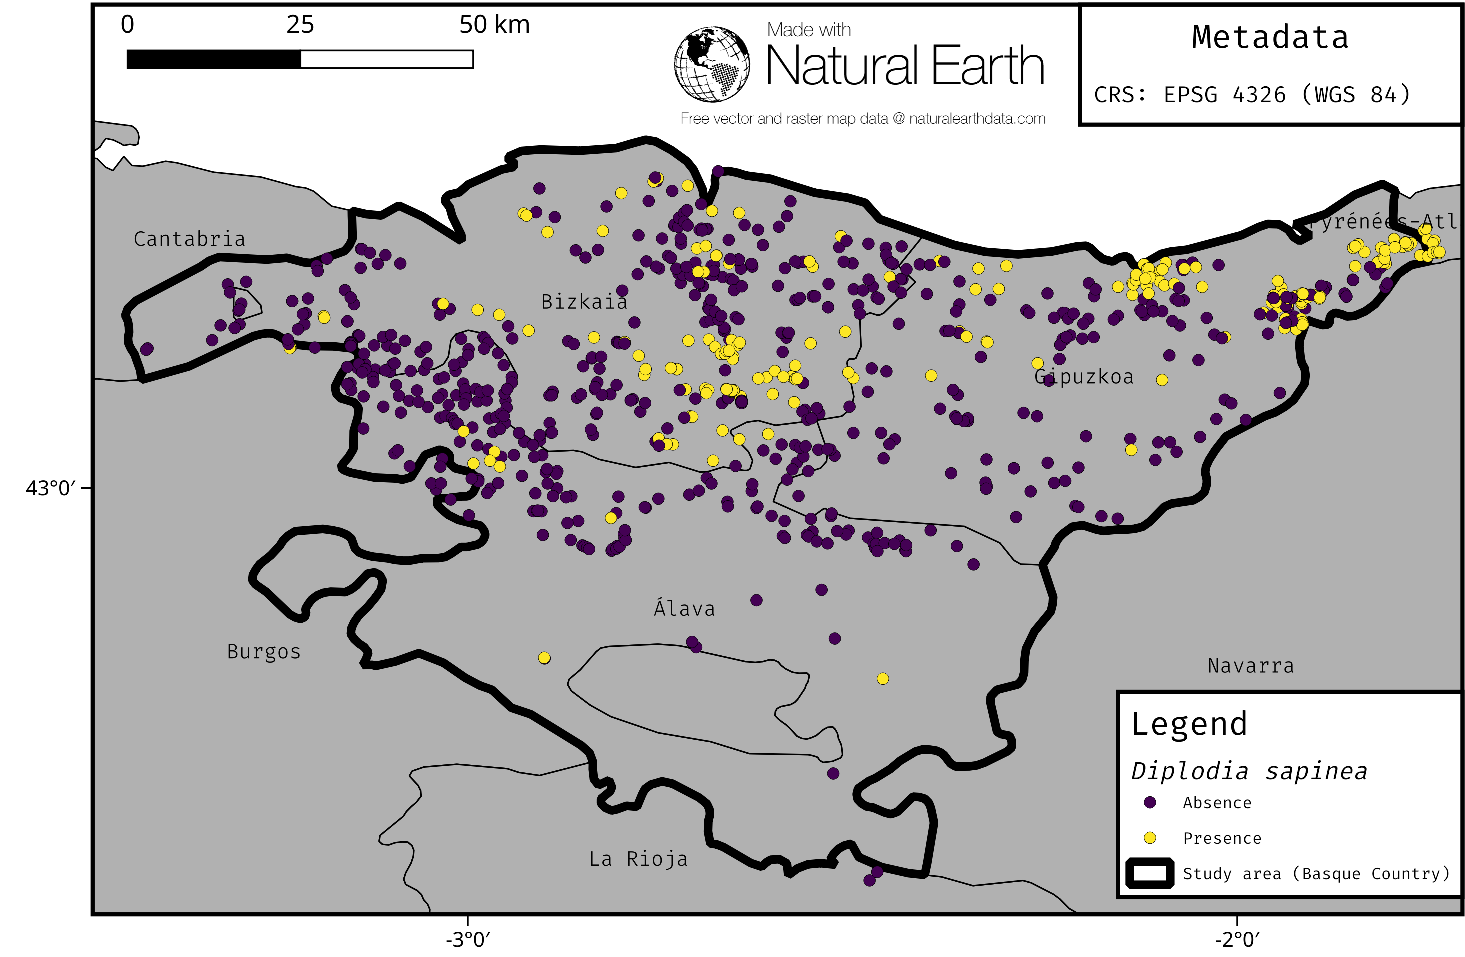
\includegraphics[width=\textwidth] {study_area.pdf}}
		\caption[Study area]{Spatial distribution of tree observations within the Basque Country, northern Spain, showing infection state by \textit{Diplodia sapinea}.}
		\label{fig: study_area}
	\end{center}
\end{figure}

\subsection{Summary of the prediction task}
This study uses parts of the dataset from \cite{Iturritxa2014}.
While \cite{Iturritxa2014} focused on the influence of environmental predictors on pathogen probability, the aim of this study is to compare different algorithms with the focus of exploring the influence of spatial autocorrelation on predictive accuracy and hyperparameter tuning.
In the present study we also introduced additional predictors (probability of hail damage at trees, soil type, lithology type, pH) to possibly enhance the predictive power of the trained models.

This particular dataset was chosen because it incorporates attributes of common geospatial modeling tasks:
An uneven distribution of the binary response variable (25/75), presence of spatial autocorrelation and predictor variables derived from various sources (previous modeling results, remote sensing data, surveyed information).
It is representative for many other ecological datasets in terms of sample size (926), number of variables (11) and predictor types (numeric as well as nominal).

\subsection{Variables}

The following (environmental) variables were used as predictors: Mean temperature (March - September), mean total precipitation (July - September), \ac{PISR}, elevation, slope (degrees), potential hail damage at trees, tree age, pH value of soil, soil type, lithology type, and the year when the tree was surveyed.
Temperature, precipitation and \ac{PISR} are long-term averages (1951 - 1999) of meteorological stations across the Iberian Peninsula \citep{Ninyerola2005}.
Tree infection caused by the fungal pathogen \textit{Diplodia sapinea} represents the response variable.
The ratio of infected and non-infected trees in the sample is roughly 1:3 (223, 703).
Precipitation, temperature and PISR were already attached to the dataset.
All other variables were extracted to the point data from their raw sources.

\cite{Iturritxa2014} showed in their study that the presence or absence of hail damage observed on trees is an important predictor when modeling pathogen infections of trees in the Basque Country.
Because almost every infected tree by \textit{Diplodia sapinea} showed hail damage, it was assumed that the pathogen uses the open wounds caused by the hail damage as an entry point.
To make the tree-based hail damage variable spatially available for the whole Basque country, we spatially predicted hail damage potential (in probabilities from 0 - 1) as a function of climatic variables using a \ac{GAM} \citep{Schratz2016}.
In the following we shortly describe the source and modifications of the new variables.
For the remaining ones, please see \cite{Iturritxa2014}.

Soil type was predicted by \cite{Hengl2017} using approx. 150.000 soil profiles at a spatial resolution of 250 m.
The age of trees was imputed and trimmed to a value of 40 to reduce the influence of outliers.
The ph value was mapped by the \cite{ph} using a regression-kriging approach based on 12.333 soil pH measurements from 11 different sources.
GeoEuskadi provided the lithology types \citep{lithology}.
The rock class were aggregated by the respective top level class for magmatic types and sub-classes for sedimentary rocks \citep{Grotzinger2016} (\autoref{table:descriptive_summary_non_numeric}).

We removed three observations due to missing information in some variables leaving a total of 926 observations (\autoref{table:descriptive_summary_numeric}).
All nominal variables (soil and lithology-type) were dummy-encoded.
To avoid introducing collinearity, the following reference levels of the dummy-encoded variables were removed from the data: soil type: "soils with clay enriched sub-soils". Lithology type: "surface deposits".

\subsection{Study area}

The Basque country in northern Spain represents the study area (\autoref{fig: study_area}).
It has a spatial extent of 7355 km\textsuperscript{2}.
Precipitation decreases towards the south while the duration of summer drought increases.
Between 1961 and 1990, mean annual precipitation ranged from 600 to 2000 mm\, with annual mean temperatures between 8 and 16\degree C \citep{Ganuza2003}.
The wooded area covers approximately 54\% of the territory (3969.62 km\textsuperscript{2}), which is one of the highest ratios in the EU.
Radiata pine is the most abundant species occupying 33.27\% of the total area \citep{Mugica2016}.

\section{Methods}

\noindent In this study we provide an exemplary analysis combining both tuning of hyperparameters (see \autoref{subsec:importance_of_tuning}) using nested \ac{CV} (see \autoref{subsubsec:nested_cv}) and the use of spatial \ac{CV} to assess bias-reduced model performance (see \autoref{subsec:spcv_pred_mod}).
We compared predictive performance using four settings: Non-spatial \ac{CV} for performance estimation combined with non-spatial hyperparameter tuning (\emph{non-spatial/non-spatial}), spatial \ac{CV} estimation with spatial hyperparameter tuning (\emph{spatial/spatial}), spatial \ac{CV} estimation with non-spatial hyperparameter tuning (\emph{spatial/non-spatial}), and spatial \ac{CV} estimation without hyperparameter tuning (\emph{spatial/no tuning}).
We used the open-source statistical programming language R \citep{R_core}.
The algorithm implementations of the following packages have been used: \textit{gbm} \citep{gbm} (\ac{BRT}, \cite{Elith2008}), \textit{mgcv} \citep{mgcv} (\ac{GAM}), \textit{kernlab} \citep{kernlab} (\ac{SVM}, \cite{Vapnik1998}), \textit{kknn} \citep{kknn} (\ac{KNN}, \cite{Dudani1976}), and \textit{ranger} \citep{ranger} (\ac{RF}, \cite{Breiman2001}). 
The spatial partitioning functions of the \textit{sperrorest} package have been integrated into the \textit{mlr} package as part of this work.
\textit{mlr} provides a standardized interface for a wide variety of statistical and machine-learning models in R simplifying essential modeling tasks such as hyperparameter tuning, model performance evaluation and parallelization \citep{bischlMlrMachineLearning2016}. 
The complete analysis including data is available as a research compendium at Zenodo (\url{https://doi.org/10.5281/zenodo.2591746}))  \citep{schratz_patrick_2019_2591746}.	

\subsection{Tuning}
\label{subsec:methods_tuning}

% parameter limits
\begin{table}[b!]
\centering
\caption[t]{Hyperparameter ranges and types for each model.
	Notations of hyperparameters from the respective R packages were used.
	Note that parameter \texttt{sp} of the GAM is a vector with eight entries (one entry for each numeric predictor). \texttt{p} is the number of predictors.}
\begingroup\footnotesize
\begin{tabular}{llllrrr}
	\\
	Algorithm (package)            & Hyperparameter             & Type    & Start     & End      & Default    \\
	\hline
	\multirow{3}{*}{BRT (gbm)}     & \texttt{n.tree}            & integer & 100       & 15000    & 100        \\
	                               & \texttt{shrinkage}         & numeric & 0         & 1.0      & 0.001      \\
	                               & \texttt{interaction.depth} & integer & 1         & 20       & 1          \\
	\midrule
	\multirow{2}{*}{KNN (kknn)}    & \texttt{k}                 & integer & 1         & 100      & 7          \\
								   & \texttt{distance}          & integer & 1         & 100      & 2          \\
								   & \texttt{kernel}            & nominal & *     &           &          \\
	\midrule
	\multirow{1}{*}{GAM (mgcv)}    & \texttt{sp}                & numeric & 0         & $10^{6}$ & -          \\
	\midrule
	\multirow{2}{*}{RF (ranger)}   & \texttt{mtry}              & integer & 1         & 11       & $\sqrt{p}$ \\
	                               & \texttt{min.node.size}     & integer & 1         & 10       & 1          \\
	                               & \texttt{sample.fraction}   & numeric & 0.2       & 0.9      & 1          \\
	\midrule
	\multirow{2}{*}{SVM (kernlab)} & \texttt{C}                 & numeric & $2^{-15}$ & $2^{15}$ & 1          \\
	                               & \texttt{$\sigma$}          & numeric & $2^{-15}$ & $2^{15}$ & 1          \\
	\bottomrule
	\multicolumn{6}{l}{* triangular, Epanechnikov, biweight, triweight, cos, inv, Gaussian, optimal}     \\
\end{tabular}
\endgroup
\label{tab:hyperparameter_limits}
\end{table}

Determining the optimal (hyperparameter) settings for each model is crucial for the bias-reduced assessment of a model's predictive power.
Hyperparameters of machine-learning algorithms need to be tuned to achieve optimal performances \citep{Bergstra2012, Duarte2017, Hutter2011}.
Often enough, parametric models do not require tuning to achieve optimal performances.
However, some (semi-)parametric algorithms (e.g. \ac{GAM}, penalized regression methods) can be optimized to possibly increase their performance.

\subsubsection{Parameter vs. hyperparameter}
For parametric models the term "parameter" is often used to refer to the regression coefficients of each predictor of a fitted model.
However, for machine-learning algorithms, the terms "parameter" and "hyperparameter" both refer to "hyperparameter" as there are no regression coefficients for these models.
In addition, the term "parameter" is often used in programming to refer to an argument of a function.
Hyperparameters determine how exactly an algorithm work and they have an influence on the final outcome. 

Hyperparameters cannot be set manually if the best performance of a model is desired. 
Automatic optimization is necessary to determine the best setting.
This optimization is done via procedures such as \textit{random search} or \textit{Bayesian optimization}.
In contrast, parameters of parametric models are estimated when fitting them to the data \citep{Kuhn2013}.

\subsubsection{Tuning method}
For hyperparameter tuning, we used \ac{SMBO} as implemented in the \textit{mlrMBO} package \citep{mlrMBO}.
At first, \textit{n} hyperparameter settings are randomly chosen from a user-defined search space.
Next, they are evaluated on the chosen resampling strategy.
Based on the previous evaluations a regression model is fitted. 
The regression model estimates the performance of the machine learning method for unknown hyperparameter settings. 
Using these estimates, a new promising hyperparameter setting is proposed to be evaluated next.
This is continued until a termination criterion is reached \citep{Hutter2011, Jones1998}.
In this work we used an initial design of 30 randomly composed hyperparameter settings and a termination criterion of 70 iterations, resulting in a total budget of 100 evaluated settings per fold.
This tuning approach substantially reduces the tuning budget that is needed to find a setting that is close to the global minimum compared to methods that do not use information from previous runs such as \textit{random search} or \textit{grid search} \citep{Bergstra2012}.

\subsubsection{Hyperparameter search spaces}
The boundaries of the hyperparameter search spaces were based on the suggestions of the \textit{mlrHyperopt} package.
In cases when the optimal setting of the folds of a model was close to the specified minimum or maximum of the tuning space, we extended the limits.
We furthermore checked on the first five inner folds of the first outer fold that the number of tuning iterations set in the \ac{SMBO} tuning was sufficiently large (\autoref{fig:optimization_paths}).
This requirement was met if no new local minimum was found in the last 10 \% of the iterations of the selected fold.

In addition, all models were fitted using their respective default hyperparameter settings, i.e. no tuning was performed.
For SVM we used $\sigma = 1$ and $C = 1$ to suppress the automatic tuning that is usually applied by the \emph{kernlab} package.
These are the default settings set by the package before the automatic tuning is applied.
The GAM implementation used in this work performs by default an internal non-spatial \ac{GCV} to find the best smoothing parameter $\lambda$ for each predictor \citep{mgcv}.
To make the optimization of models comparable, we tuned $\lambda$ for each covariate using the tuning method that was also applied to the machine-learning algorithms.
For the "no tuning" setups, we set $\lambda = 0$ for all predictors.
The basis dimension for all GAM setups was set to $k = 15$ for all variables.
The search space for $\lambda$ ($0 - 10^{6}$) was determined by examining the results of a prior tuning using the internal tuning of the GAM.

\subsubsection{Spatial vs. non-spatial hyperparameter tuning}
Hyperparameters estimated from a non-spatial tuning lead to fitted models which are more adapted to the training data than models with hyperparameters estimated from a spatial tuning.
In a non-spatial tuning setting, hyperparameters that lead to a close fit of the algorithm to the data will be favored in the tuning process due to the presence of spatial autocorrelation.

Models fitted with hyperparameters from a non-spatial tuning can potentially benefit from the remaining spatial autocorrelation in the train/test split (even if a spatial resampling was used) during performance estimation and achieve a better performance than models tuned using a spatial resampling.
However, depending on the dataset structure and closeness of the model fit on the data, the reverse effect might occur and models fitted with a spatial tuning setting might yield better results.
In the end it depends on whether the training/test difference is more similar to a spatial tuning setting (i.e. more heterogeneous train/test splits) or to a non-spatial tuning setting (i.e. more homogeneous train/test sets).

\subsubsection{Practical implementation}
Most packages offering \ac{CV} solutions in R offer only random partitioning methods, assuming independence of the observations.
Package \textit{mlr}, which was used as the modeling framework in this work, was missing spatial partitioning functions but provides a unified framework for modeling and simplifies hyperparameter tuning.
Within the works of this study we implemented the spatial partitioning methods of package \textit{sperrorest} into \textit{mlr}.

\begin{figure} [t!]
	\begin{center}
		\makebox[\textwidth]{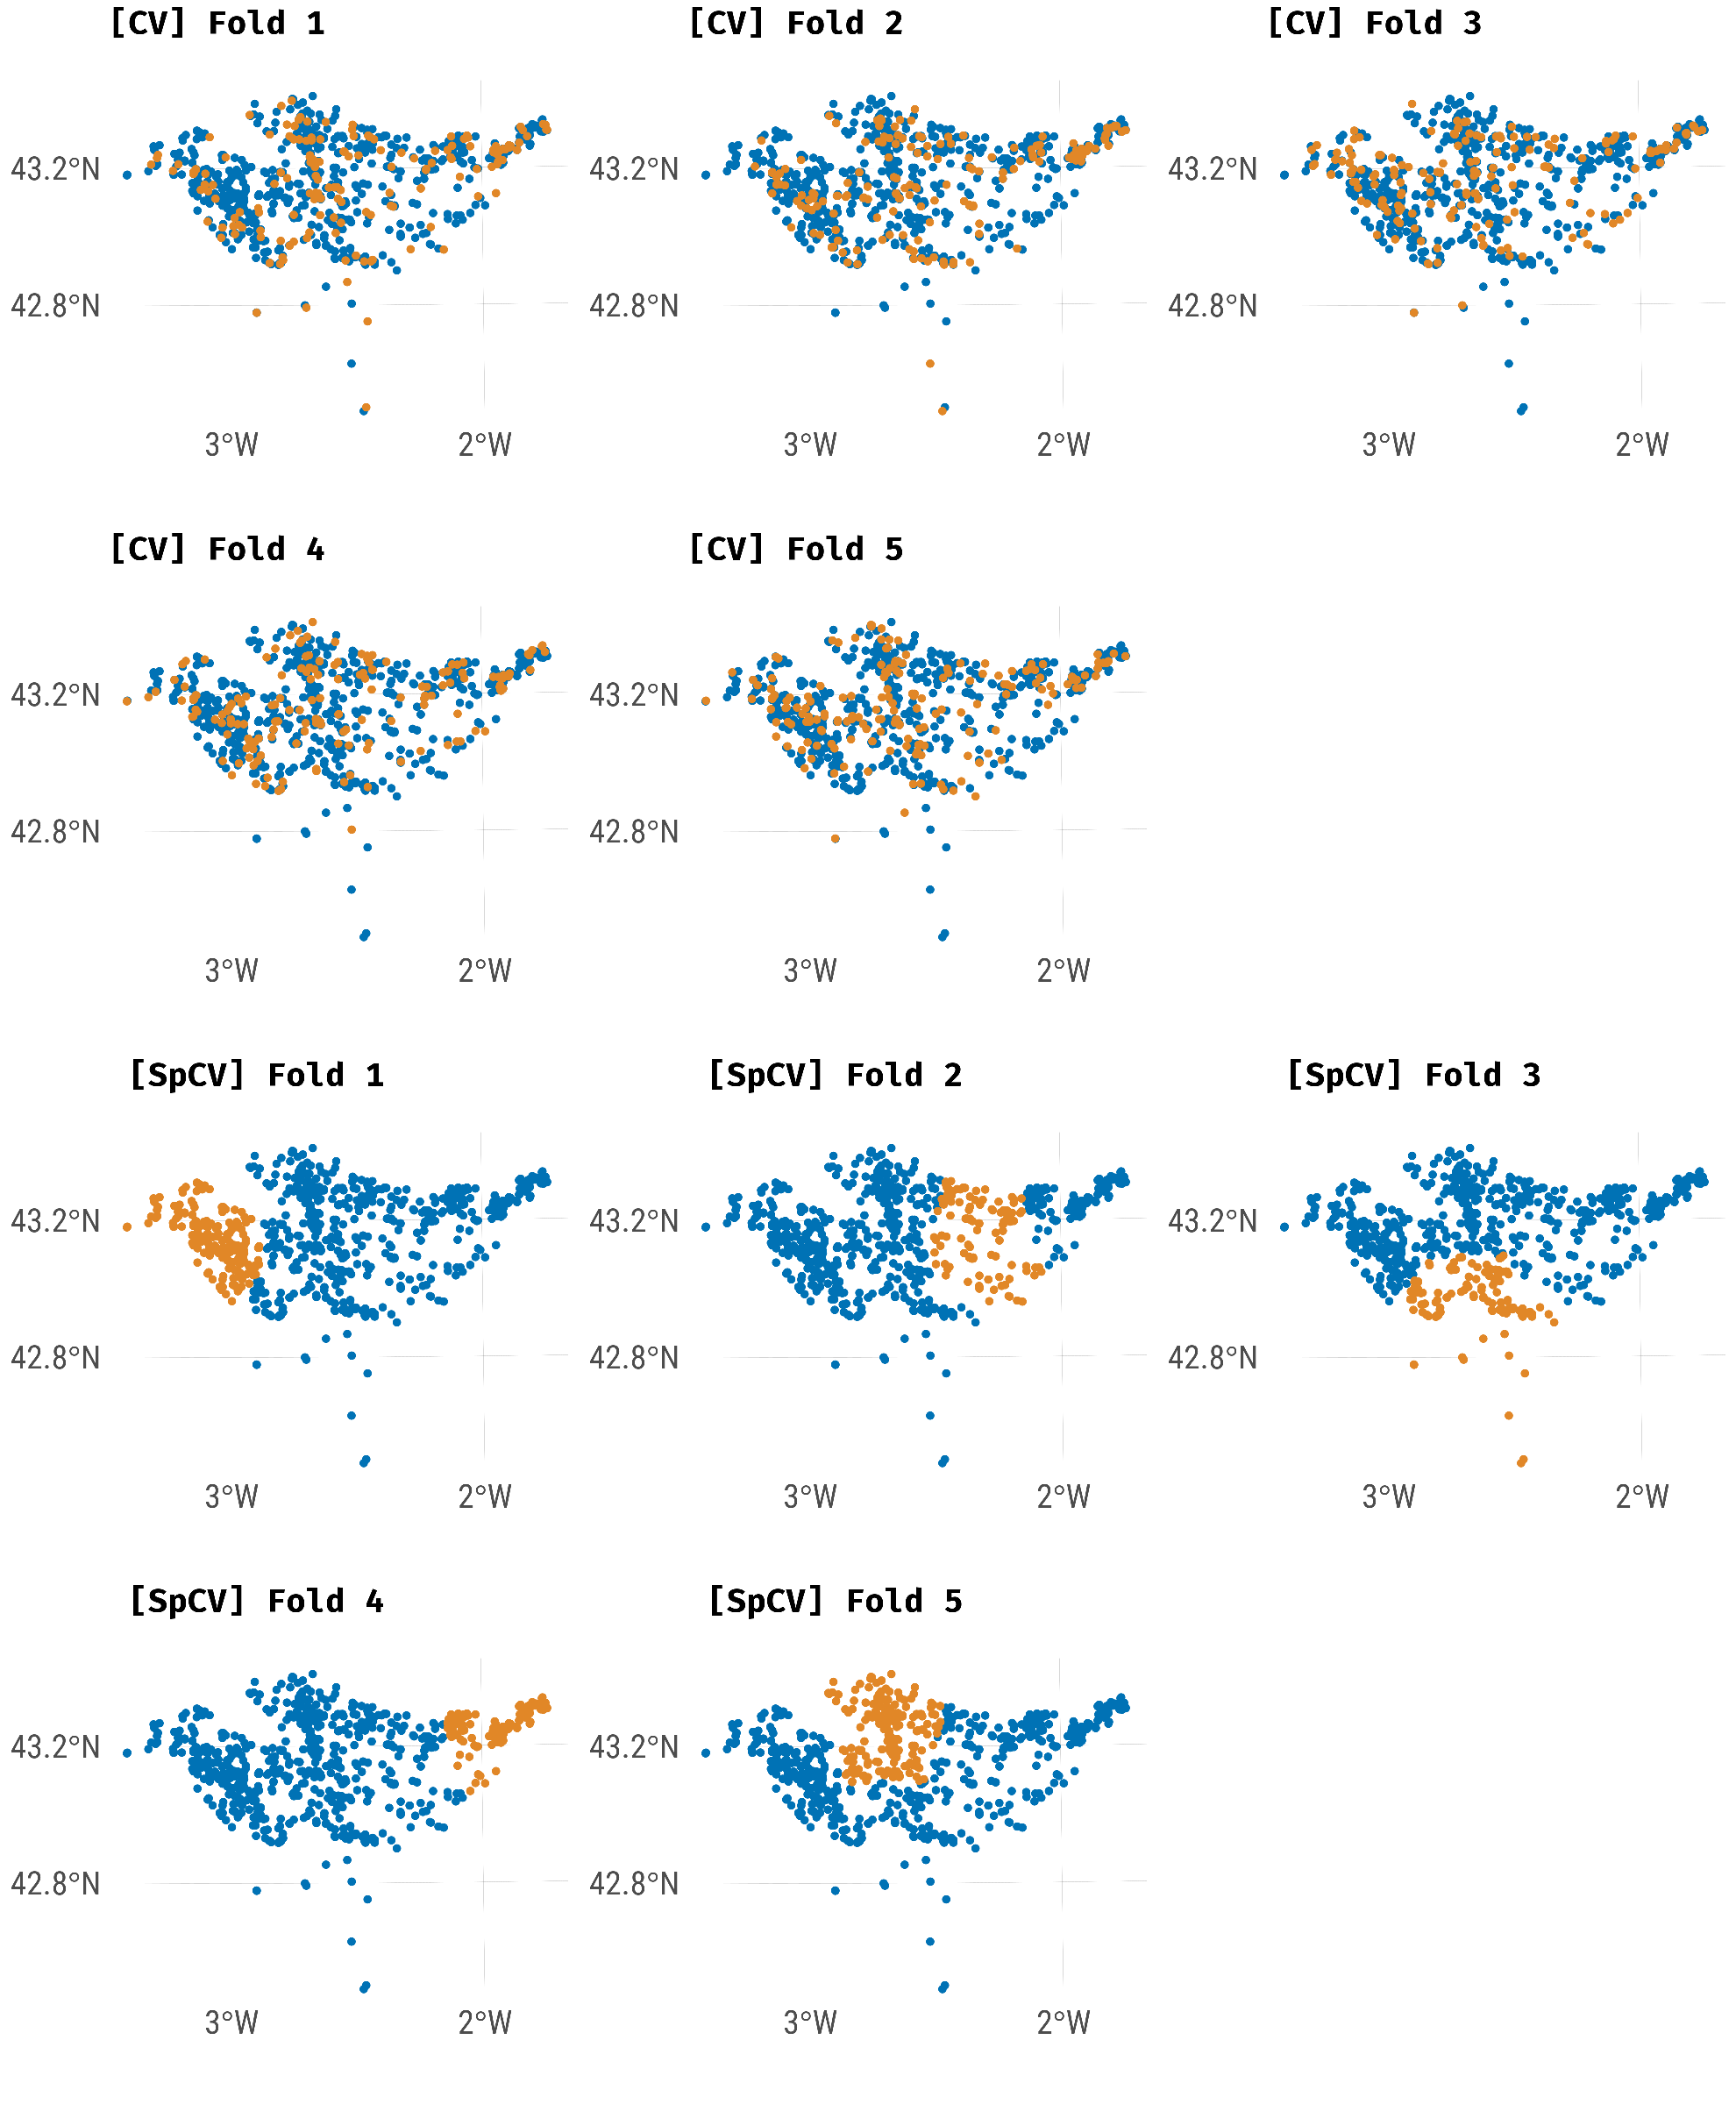
\includegraphics[height = 0.82\textheight] {spcv_nspcv_folds.pdf}}
		\caption[]{Comparison of spatial and non-spatial partitioning of the first five folds in spatial and non-spatial cross-validation performance estimation.
			Blue dots represent the training samples and orange dots the testing sample.
			"SpCV" stands for spatial cross-validation (spatial sampling of observations) and "CV" for cross-validation (random sampling of observations).}
		\label{fig:cv_settings_comparison}
	\end{center}
\end{figure}

\subsection{Estimation of predictive performance}
\label{sec:nested_cv}

\subsubsection{Nested cross-validation}
\label{subsubsec:nested_cv}
Cross-validation is a resampling-based technique for the estimation of a model's predictive performance \citep{James2013}.
The basic idea behind \ac{CV} is to split an existing dataset into training and test sets using a user-defined number of partitions (\autoref{fig:nested_cv}).
First, the dataset is divided into $k$ partitions or folds.
The training set consists of $k - 1$ partitions and the test set of the remaining partition.
The model is trained on the training set and evaluated on the test partition.
A repetition consists of $k$ iterations for which every time a model is trained on the training set and evaluated on the test set.
Each partition serves as a test set once.

\subsubsection{Influence of spatial autocorrelation in cross-validation}
In ecology, observations are often spatially dependent \citep{Dormann2007, Legendre1989}.
Subsequently, they are affected by underlying spatial autocorrelation by a varying magnitude \citep{Legendre1993, Cliff1970, Telford2005}.
Model performance estimates are expected to be overoptimistic due to the similarity of training and test data in a non-spatial partitioning setup when using any kind of cross-validation for tuning or validation \citep{Burman1994, Cliff1970, Racine2000}.
Therefore, cross-validation approaches that adapt to this problem should be used in any kind of performance evaluation when spatial data is involved \citep{Meyer2018, Telford2009}.
In this work we use the spatial cross-validation approach after \cite{sperrorest} which uses $k$-means clustering to reduce the influence of spatial autocorrelation.
In contrast to non-spatial CV, spatial CV reduces the influence of spatial autocorrelation by partitioning the data into spatially disjoint subsets (\autoref{fig:nested_cv}).

A 100 times repeated (to reduce random variability introduced by partitioning) five-fold partitioning setting was chosen for performance estimation (\autoref{fig:nested_cv}).
For hyperparameter tuning, again five folds were used to partition the training set of each fold.
Hyperparameter tuning only applied to the machine-learning algorithms.
A sequential model-based optimization approach was used for optimization (see \autoref{subsec:methods_tuning}).
Model performances of every hyperparameter setting were computed at the tuning level and averaged across folds.
The hyperparameter setting with the lowest mean Brier score across all tuning folds was used to train a model on the training set of the respective performance estimation level.
This model was then evaluated on the test set of the respective fold (performance estimation level).

\subsubsection{Cross-Validation settings}

To underline the crucial need for spatial \ac{CV} when assessing a model's performance, and to identify overoptimistic outcomes when neglecting to do so, we used the following CV setups:

\begin{itemize}
	\item Nested non-spatial \ac{CV} which uses random partitioning and non-spatial hyperparameter tuning (\emph{non-spatial/non-spatial})
	\item Nested spatial \ac{CV} which uses k-means clustering for partitioning \citep{Brenning2005} and results in a spatial grouping of the observations in combination with non-spatial hyperparameter tuning (\emph{spatial/non-spatial})
	\item Sested spatial \ac{CV} including spatial hyperparameter tuning (\emph{spatial/spatial}) 
	\item Spatial \ac{CV} without hyperparameter tuning (\emph{spatial/no tuning})
	\item Non-spatial \ac{CV} without hyperparameter tuning (\emph{non-spatial/no tuning})
\end{itemize}

\noindent Setup (\emph{non-spatial/non-spatial}) was only used to show the overoptimistic results when using non-spatial \ac{CV} with spatial data and setups \emph{spatial/non-spatial}, \emph{spatial/spatial} to reveal the differences between spatial and non-spatial hyperparameter tuning.
Setup (\emph{spatial/spatial}) should be used when conducting spatial modeling with machine learning algorithms that require hyperparameter tuning.

\subsubsection{Performance measure}
Brier score was selected as a scoring rule to to compare the predictive performances of all algorithms \citep{Brier1950}.
In contrast to other commonly used measures for binary classification (e.g. the \ac{AUROC}), Brier score classifies as a proper scoring rule \citep{Byrne2016, Gneiting2007}.
It is defined as the mean quadratic loss between the predicted and observed probabilities.
It ranges from 0 to 1 with low values indicating a good prediction \citep{Brier1950}.

\subsubsection{A note on spatial autocorrelation structures in parametric models}
In this work we assume that, on average, the predictive accuracy of parametric models with and without spatial autocorrelation structures incorporated into the model is the same.
However, there is little research on this specific topic \citep{Dormann2007b, Mets2017} and a detailed analysis goes beyond the scope of this work.
In our view, a possible analysis would need to estimate the spatial autocorrelation structure of a model for every fold of a cross-validation using a data-driven approach (i.e. automatically estimate the spatial autocorrelation structure from each training set in the respective CV fold) and compare the results to the same model fitted without a spatial autocorrelation structure.
Since we only focused on predictive accuracy in this work, we did not use spatial autocorrelation structures during model fitting for \ac{GLM} and \ac{GAM} to reduce runtime.

\begin{figure} [t!]
	\begin{center}
		\makebox[\textwidth]{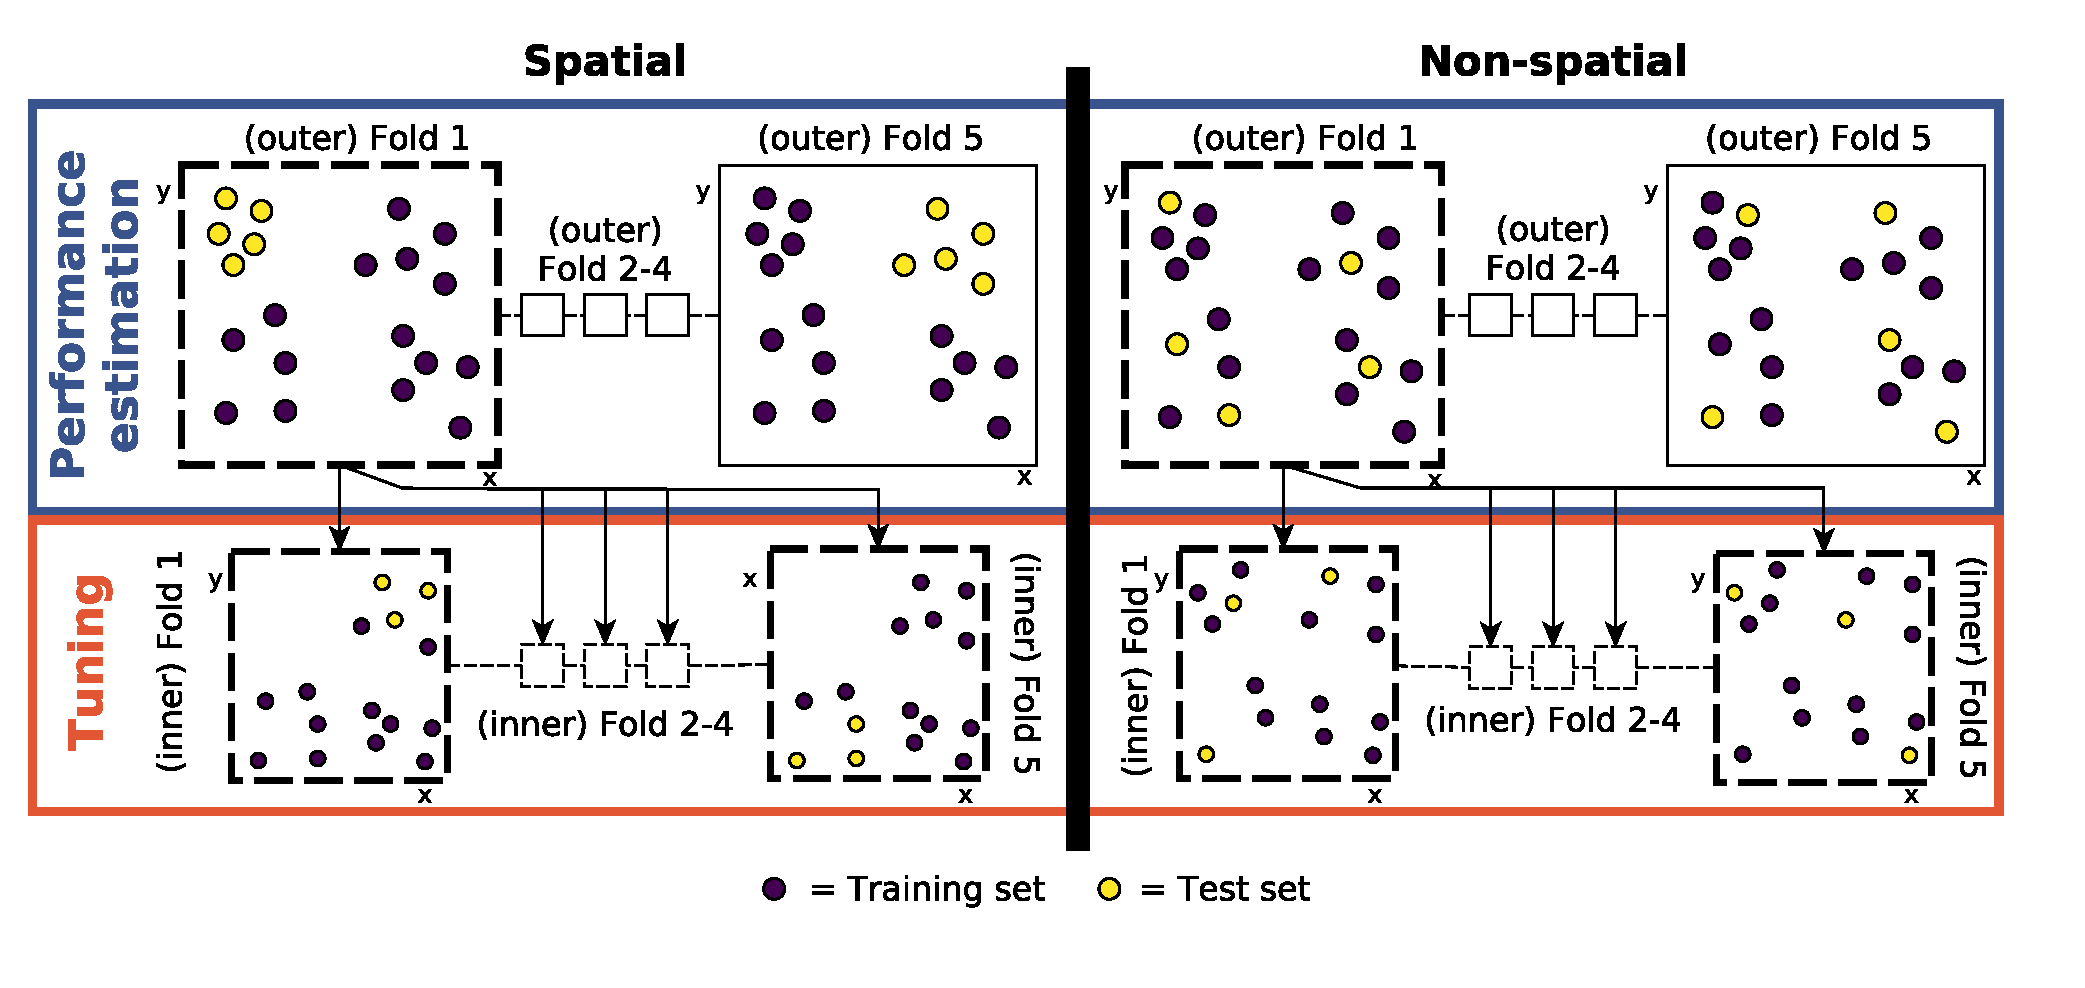
\includegraphics[width=\textwidth] {cross-validation_farbig.pdf}}
		\caption[]{Theoretical concept of spatial and non-spatial nested cross-validation using five folds for hyperparameter tuning and performance estimation.
			Yellow/purple dots represent the training and test set for performance estimation, respectively.
			The tuning sample is based on the respective performance estimation fold sample and consists again of training (orange) and test set (blue).
			Although the tuning folds of only one fold are shown here, the tuning is performed for every fold of the performance estimation level.}
		\label{fig:nested_cv}
	\end{center}
\end{figure}

\section{Results}

\subsection{Tuning}

\begin{figure} [t!]
	\begin{center}
		\makebox[\textwidth]{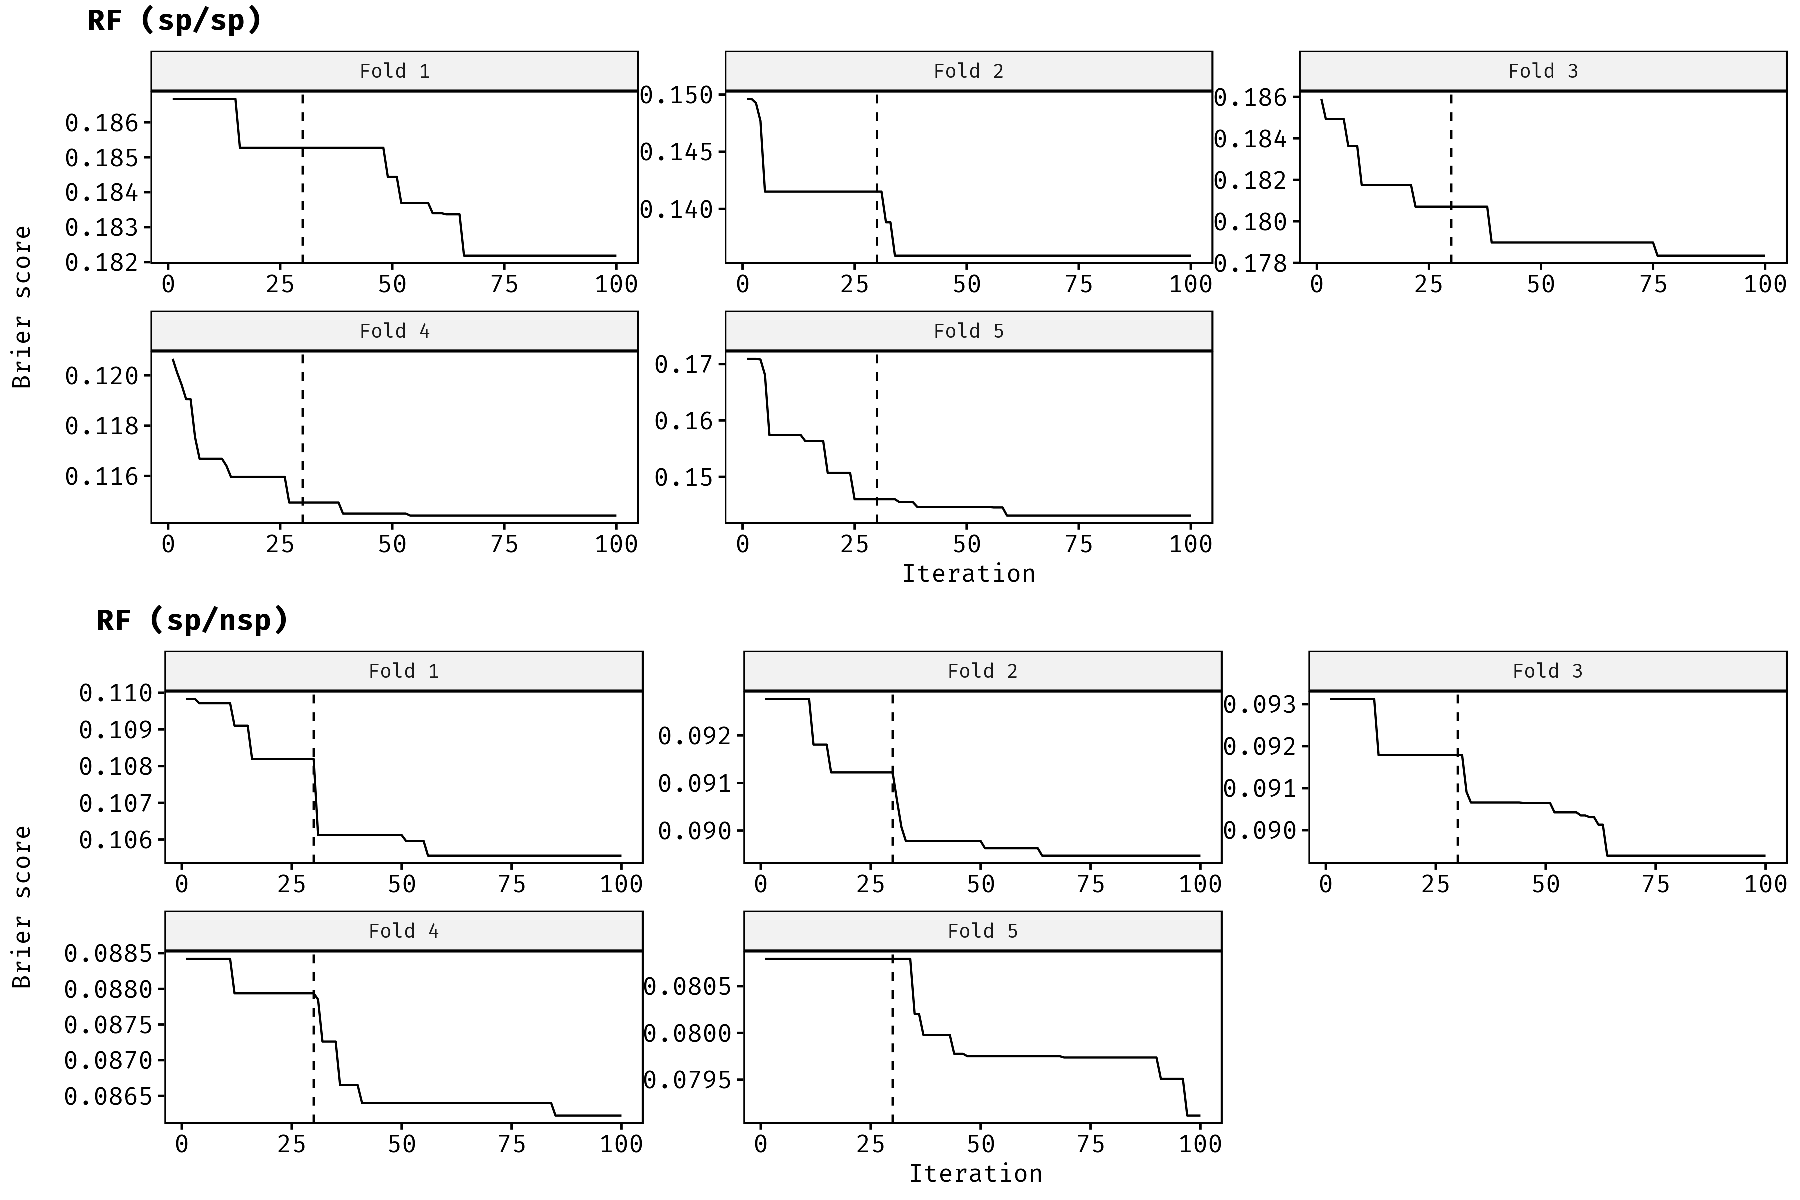
\includegraphics[width=\textwidth] {opt-paths-RF-sp-vs-nsp.pdf}}
		\caption[]{SMBO optimization paths of the first five folds of the \emph{spatial/spatial} and \emph{spatial/non-spatial} CV setting for \ac{RF}. The dashed line marks the border between the initial design (30 randomly composed hyperparameter settings) and the sequential optimization part in which each setting was proposed using information from the prior evaluated settings. Optimization paths of the remaining models can be found in the appendix.}
		\label{fig:optimization_paths}
	\end{center}
\end{figure}

\subsubsection{Optimization paths}
To proof the effectiveness of the tuning, the optimization paths of the first five folds of RF for settings {spatial/spatial} and \emph{spatial/non-spatial} are visualized (\autoref{fig:optimization_paths}).
Using 100 SMBO iterations, all shown folds show decrease in Brier score along the optimization path (\autoref{fig:optimization_paths}).
Apart from fold 5 of setting \emph{spatial/non-spatial}, all folds show a saturation of at least 15 or more iterations in which no new local minimum was found.

\subsubsection{Best hyperparameter settings}
There were notable differences in the distribution of the estimated optimal hyperparameters between the spatial (\emph{spatial/spatial}) and non-spatial (\emph{spatial/non-spatial}, \emph{non-spatial/non-spatial}) tuning settings (\autoref{fig:best_parameter_combs}): In the spatial tuning setting, all models besides BRT show a wide range of optimal hyperparameters across folds.
By contrast, the range of optimal settings in the non-spatial tuning case is much smaller and often clusters around a few specific settings (e.g. compare the spatial and non-spatial results of the SVM) (\autoref{fig:best_parameter_combs}).

For the spatial tuning case of RF, the estimated \texttt{$m_{try}$} values mainly ranged between 1 and 3 and \texttt{$m_{try}$} of 1 was most often the optimal value.
This stands in strong contrast to the non-spatial tuning setting in which \texttt{$m_{try}$} mainly ranged between 3 and 5 and \texttt{$m_{try}$} of 3 was most often the optimal choice.
Generally, we observed the tendency that spatially tuned hyperparameters are often close to the limits of the search space especially when compared to their non-spatial counterparts.
The GAM results are not included in \autoref{fig:best_parameter_combs} as the estimated hyperparameter (smoothing parameter $\lambda$) is a vector of length eight (eight being the number of non-linear variables in the model formula) that cannot be visualized in a 2D space.

\subsection{Predictive performance}
\label{subsec:pred_perf}

\subsubsection{Which models showed the best performance?}
For the spatial settings (\emph{spatial/spatial} and \emph{spatial/no tuning}), \ac{RF} showed the best predictive performance followed by BRT, KNN and GLM (\autoref{fig:cv_final_boxplots}).
The absolute difference between the best (RF) and worst (GAM) performing model in our benchmark comparison is 0.039 (mean Brier score (\emph{spatial/spatial})).
The GAM showed a high variance for all spatial settings compared to all other algorithms.

\subsubsection{Effect of hyperparameter tuning on predictive performance}
The tuning of hyperparameters resulted in a clear increase of predictive performance for BRT (0.183 (\emph{spatial/spatial}) vs. 0.201 (\emph{spatial/no tuning}) mean Brier score), GAM (0.206 (\emph{spatial/spatial}) vs. 0.251 (\emph{spatial/no tuning}) and KNN (0.181 (\emph{spatial/spatial}) vs 0.210 (\emph{spatial/no tuning}) mean Brier score) (\autoref{fig:cv_final_boxplots}).
No effect of hyperparameter tuning on predictive performance was visible for RF and SVM.
The use of spatial partitioning in hyperparameter tuning (setting (\emph{spatial/spatial}) had an substantial positive impact for BRT and a negative one for GAM and KNN (\autoref{fig:cv_final_boxplots}).

\begin{figure} [H]
	\begin{center}
		\makebox[\textwidth]{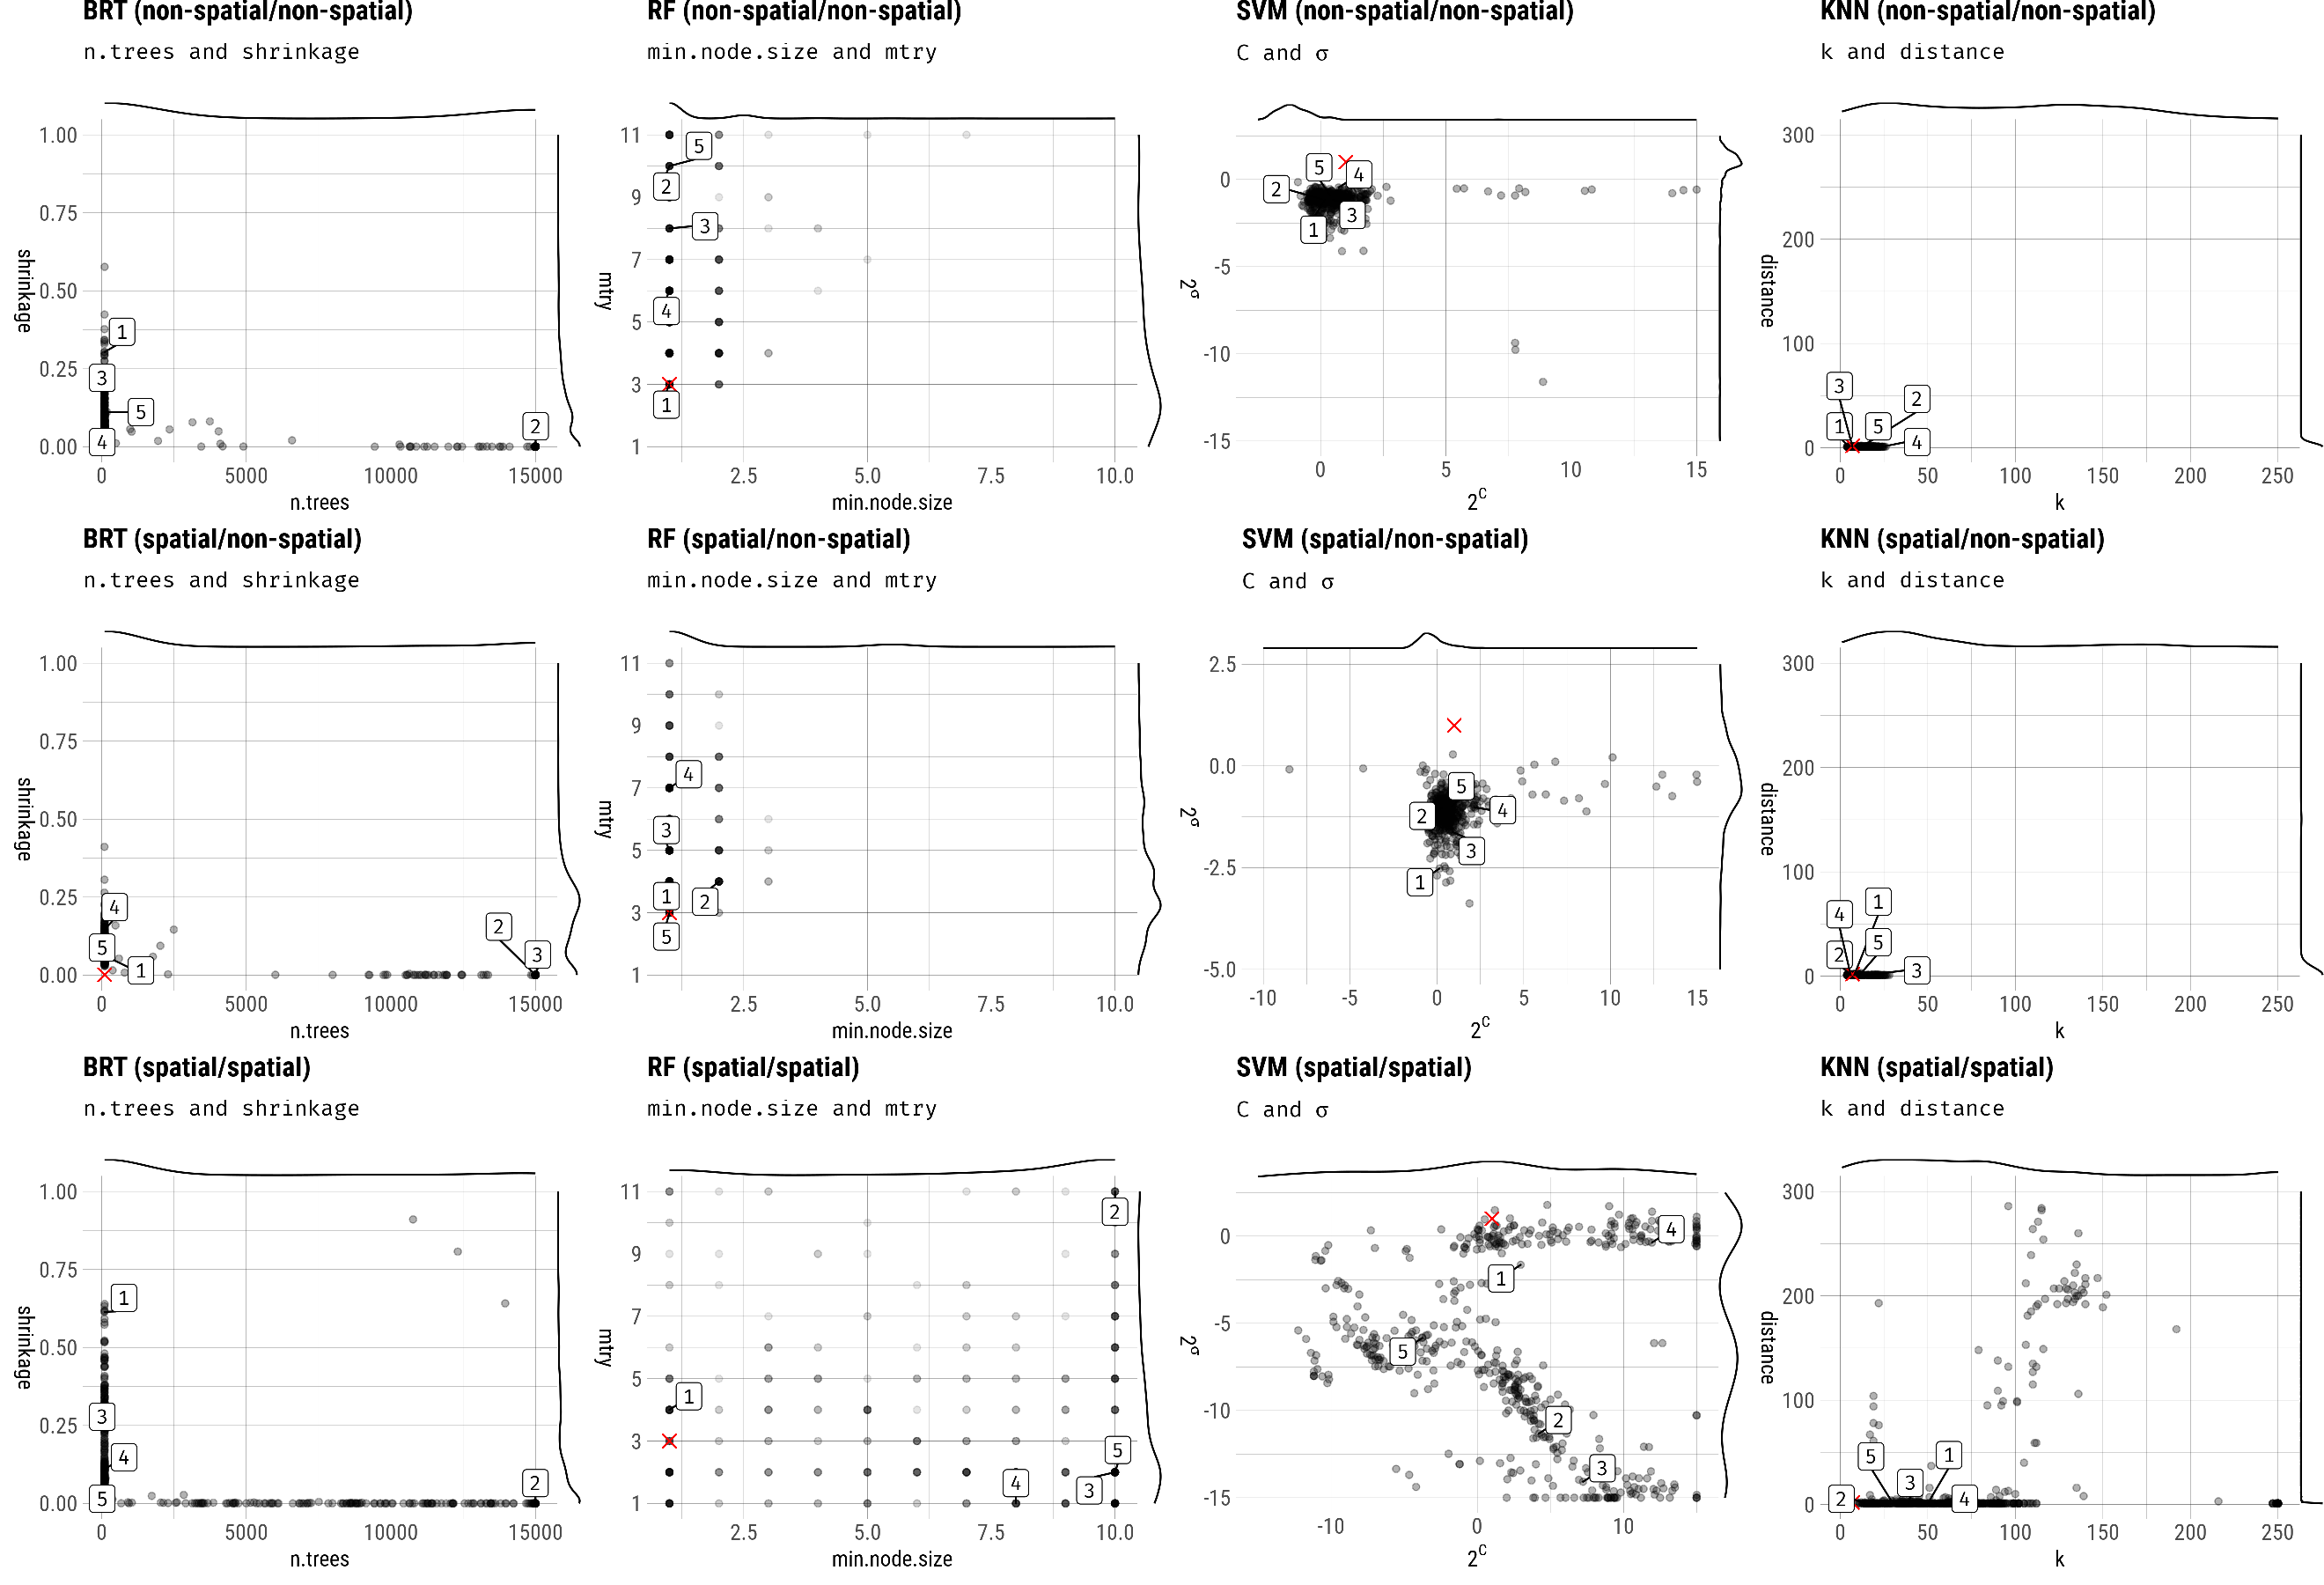
\includegraphics[angle=90, height = 0.85\textheight] {tuning_effects_all_models_mbo.pdf}}
		\caption[]{Best hyperparameter settings by fold (500 total) each estimated from 100 (30/70) SMBO tuning iterations per fold using five-fold cross-validation. 
		Split by spatial and non-spatial partitioning setup and model type.
			Red crosses indicate the default hyperparameters of the respective model.
			Black dots represent the winning hyperparameter setting of each fold.
			The labels ranging from one to five show the winning hyperparameter settings of the first five folds.
			Density lines on both axis show the density distribution of the respective variable.}
		\label{fig:best_parameter_combs}
	\end{center}
\end{figure}

\subsubsection{Comparison of spatial vs non-spatial tuning}
Predictive performance estimates based on non-spatial partitioning (\emph{non-spatial/non-spatial} or \emph{non-spatial/no tuning}) are around 33 - 47\% higher, i.e. overoptimistic, compared to their spatial equivalents (\emph{spatial/spatial}, \emph{spatial/no tuning}).
BRT and RF show the highest differences between these two settings (47\% and 46\%, respectively) while GLM was the least affected (33\%).

\begin{figure} [t!]
	\begin{center}
		\makebox[\textwidth]{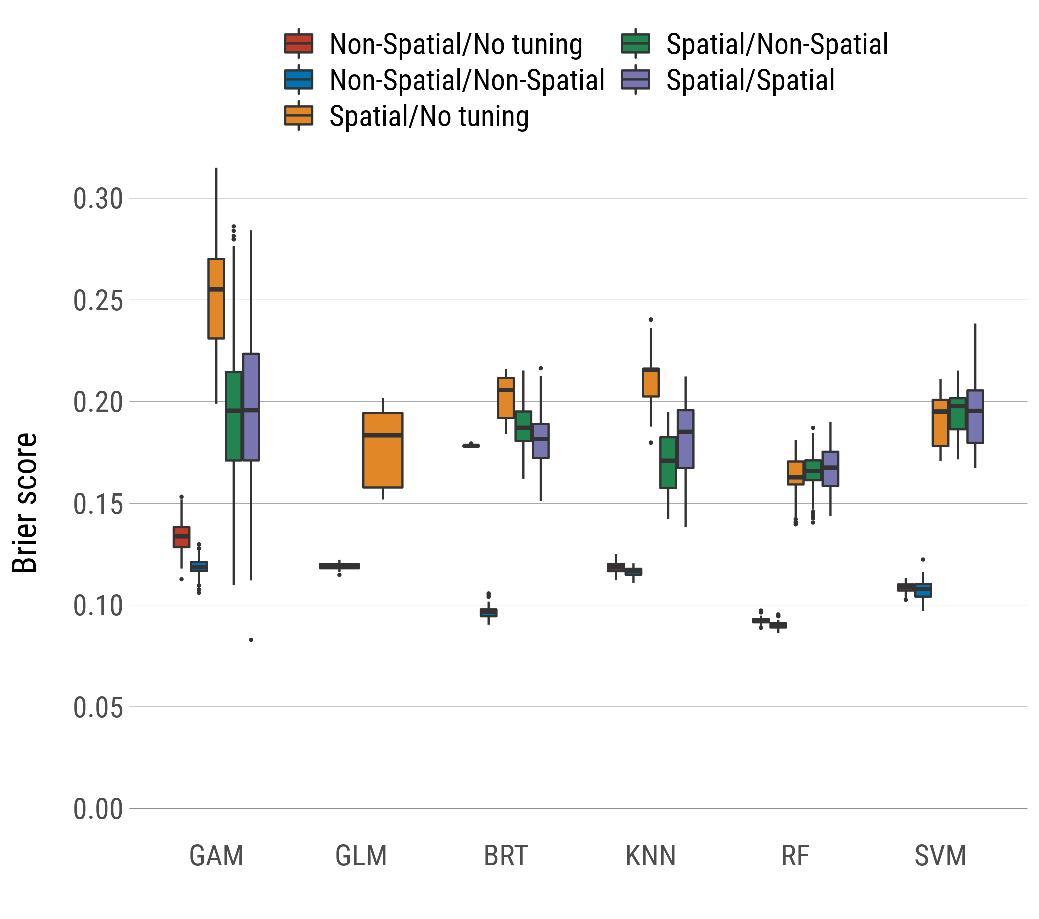
\includegraphics[width=\textwidth] {cv_boxplots_final_brier.pdf}}
		\caption[]{(Nested) \ac{CV} estimates of model performance at the repetition level using 100 SMBO iterations for hyperparameter tuning.
			CV setting refers to performance estimation/hyperparameter tuning of the respective (nested) CV, e.g. "Spatial/Non-Spatial" means that spatial partitioning was used for performance estimation and non-spatial partitioning for hyperparameter tuning.}
		\label{fig:cv_final_boxplots}
	\end{center}
\end{figure}

\section{Discussion}
\label{sec:discussion}

\subsection{Tuning}

\subsubsection{Tuning methods} 
The question on the most efficient approach of hyperparameter tuning has been discussed for decades \citep{Bengio2000, Probst2018a, Yang2017}.
The goal is to use as few computational resources as possible to find a nearly optimal hyperparameter setting of an algorithm for a specific dataset.
In this respect, methods like \textit{random search} are particularly promising in multidimensional hyperparameter spaces with possibly redundant or insensitive hyperparameters (low effective dimensionality; \citep{Bergstra2012}).
Adaptive search algorithms offer computationally efficient solutions to these difficult global optimization problems in which little prior knowledge on optimal subspaces is available.
Approaches like Bayesian Optimization and F-racing are widely used for optimization of black-box models \citep{Birattari2002, mlrMBO, Brochu2010, Malkomes2016}.
In this study, we used a sequential model-based optimization (Bayesian optimization) method.
Other tuning methods would have yielded almost identical results but at the cost of increased computational efficiency and less robustness in terms of finding the local minimum.

\subsubsection{Algorithm sensitivity to tuning}
Some models (e.g. \ac{RF}) are known to be relatively insensitive to hyperparameter tuning \citep{Probst2018b}.
However, as the effect of hyperparameter tuning also depends on the dataset, hyperparameters should always be tuned.
If no tuning is conducted, it cannot be ensured that the respective model showed its best possible predictive performance on the dataset.

\subsubsection{Hyperparameter search spaces}
Computational expense, especially when using tuning methods like random search, should focus on plausible parameter settings for each model.
It should be ensured by visual inspection that the majority of the obtained optimal hyperparameter settings is not close to the ranges of the tuning space.
If the optimal hyperparameter settings are clustered at the borders of the parameter search space, this implies that optimal hyperparameters may actually lie outside the given range.
However, extending the tuning space is not always possible nor practical as (1) numerical problems within the algorithm may occur that may prohibit further extension of the tuning space; (2) some algorithms tend to mainly use the limits of the given search space although no significant increase is achieved (e.g. KNN in the \emph{spatial/spatial} setting).

We encountered exactly these problems in the \emph{spatial/spatial} setting for BRT, KNN and SVM.
For example, in the \emph{spatial/spatial} setting, we should have further increased the search space for the mentioned models based on the distribution of the optimal hyperparameters of each fold (\autoref{fig:best_parameter_combs}).
However, using the extended setting, the algorithms did not converge anymore for some folds and at the same time runtime increased without a significant increase in predictive performance.

All these points show the need for a thorough specification of parameter search spaces.
As the optimal hyperparameter ranges also depend on the dataset characteristics, it is not possible to define a universal search space that works best on every dataset.
Nevertheless, the chosen hyperparameter limits of this work can serve as a starting point for future analyses in the spatial modeling field.
Within the framework of the \textit{mlr} project a database exists which stores hyperparameter settings of various models from users that can serve as a reference point \citep{mlrhyperopt}.

\subsubsection{Comparison of spatial vs non-spatial tuning}
No major differences in model performances were found when using spatial versus non-spatial hyperparameter tuning procedures (e.g. 0.019 for \ac{BRT} (0.182 vs. 0.201 mean Brier score).

The winning algorithm RF is used to discuss the optimal estimated hyperparameters per fold of the spatial and non-spatial tuning setting in more detail.
Although the tuning of RF had no substantial effect on predictive performance (\autoref{fig:cv_final_boxplots}), the estimated optimal hyperparameters of RF differ for the non-spatial and spatial tuning setting (\autoref{fig:best_parameter_combs}).
We split the following discussion into two points: (1) The nature of the algorithm and (2) the implications which method should be chosen.
(1) In a non-spatial tuning setting, RF will prioritize spatially autocorrelated predictors because these will yield the best performance results in the internal variable selection process that uses the \textit{Gini impurity measure} \citep{Biau2016, Gordon1984}. 
We define "spatially autocorrelated predictors" as variables that show highly similar patterns in its relationship to the response in both training and test set.
By selecting these, the algorithm is able to achieve good performances because the trained patterns appear almost identical in the test set. 
The resulting performances are then overoptimistic as they benefit highly from the non-spatial sampling scheme.

In this pre-selection, \texttt{mtry} values around 3 - 5 are favored because they provide a fair chance of having one of the autocorrelated predictors included in the selection.
At the same time, \texttt{mtry} is low enough to prevent overfitting on the training data because the autocorrelated predictors are not always available to the algorithm.

In the spatial tuning setting, mainly \texttt{mtry = 1} is chosen.
This specific value essentially removes the internal variable selection process by \texttt{mtry} as RF is forced to use the predictor that was randomly assigned.
Subsequently, on average, each predictor will be chosen equally often and the higher weighting of spatially autocorrelated predictors in the final model (by choosing them more often in the trees) does not apply.
This leads to a more general model that apparently performs better on heterogeneous datasets (e.g. if training and test data are less affected by spatial autocorrelation) as it is the case in a spatial sampling.

(2) Even though the estimated hyperparameters from a spatial and non-spatial sampling differ, they roughly achieve the same performance when being evaluated at the performance estimation level of the CV. 
This outcome is not generalizable and highly depends on the dataset of this study. 
It needs to be verified by using other spatial datasets.
Performance differences might be more substantial when using either \texttt{mtry = 1} or \texttt{mtry = 3} on datasets with different characteristics.
This applies also to all other algorithms used in this study.
In addition, if a model is going to be evaluated on a specific sampling scheme (here spatial sampling), we see no valid argument why its hyperparameters should be trained on a different sampling scheme if the predictive performances do not differ significantly.

\subsection{Predictive Performance}

\subsubsection{Non-spatial vs. spatial CV}
Our findings agree with previous studies in that non-spatial performance estimates appear to be substantially "better" than spatial performance estimates \citep{Meyer2018, Micheletti2013, Roberts2017}.
However, this difference can be attributed to an overoptimistic bias in non-spatial performance estimates in the presence of spatial autocorrelation \citep{Goetz2015, Meyer2018, Russ2010a, Steger2016}.
Spatial cross-validation is therefore required for performance estimation in spatial predictive modeling, and similar grouped cross-validation strategies have been proposed elsewhere in environmental as well as medical contexts to reduce bias in predictive performance \citep{Brenning2008, Meyer2018, Pena2015, Pohjankukka2017, Roberts2017}. 

\subsubsection{The effect of hyperparameter tuning on predictive accuracy}
Although hyperparameter tuning certainly increases the predictive performance for some models (e.g. BRT, GAM and KNN) in our case, the magnitude always depends on the meaningful/arbitrary defaults of the respective algorithm and the characteristics of the dataset.
Naturally, the tuning effect is higher for models without meaningful defaults (such as BRT and KNN) than for models with meaningful defaults such as RF.
To underline this statement, there was basically no tuning effect for SVM in this study (\autoref{fig:cv_final_boxplots}) although the SVM usually shows substantial increases when being tuned \citep{Rojas_Dominguez2018}.

\subsubsection{Predictive performance across algorithms}
Other studies also found that RF showed the best predictive performance (referring to setting \emph{spatial/spatial}) \citep{Bahn2012, Jarnevich2017, Smolinski2016, Vorpahl2012}.
The fact that the GLM is showing a better performance than the GAM shows the heterogeneous train/test split introduced by spatial partitioning: The GAM is not able to generalize enough (i.e. it overfits on the training set) if the test set is substantially different to the training set.
The high variance of the GAM performances in the spatial setting verify this: If the training set is somewhat similar to the test set, the GAM is able to achieve Brier score results around 0.19. 
In cases where training and test set are more heterogeneous, the predictive performance shows Brier score estimates up to 0.30. 
Overall, the linear approach of the GLM is able to generalize better in this study and subsequently results in a better performance.

It maybe surprising at first that the GLM is showing a showing a performance which is similar to that of BRT, KNN and SVM.
This is most likely due to the ability of the algorithm to generalize.
Highly flexible algorithms have a tendency to overfit when the test set differs substantially from the training set. 
For instance, a test set located close to the sea might be hard to predict for models trained on data that was almost exclusively located in mountainous regions. 
In such a setting, a low degree of flexibility will result in better predictions. 
This example also shows the importance of traditional parametric approaches in ecological modeling: Often enough ecological datasets show a high degree of diversity and machine-learning models might suffer from overfitting.
In this case, the interpretability, speed and generalization attributes of a GLM make this algorithm a valid choice, especially if the differences in predictive accuracy compared to black-box models is small.

\subsubsection{The influence of the performance measure}
The choice of the scoring rule for the evaluation of binary classifications is an important decision \citep{Gneiting2007}.
Measures that are not classified as "proper" can lead to undetected deviations during scoring that can end up in biased results \citep{Byrne2016}.
One of the most used performance measures in the field of binary classification, the \ac{AUROC}, is affected by this.
In a previous version of this work we used \ac{AUROC} to rank the algorithms which had the effect of GAM showing a similar performance as RF. 
So by only changing the measure, GAM went from the best (AUROC) to the worst (Brier score) algorithm.
This example highlights the importance of selecting a measure for benchmarking purposes that is classified as a proper scoring rule.
However, analyzing the effect of different measures on benchmarking performance across algorithms exceeds the scope of this work.

\subsubsection{A note on spatial autocorrelation structures in parametric models}
In this work we assume that, on average, the predictive accuracy of parametric models with and without spatial autocorrelation structures is the same.
However, there is little research on this specific topic \citep{Dormann2007b, Mets2017} and a detailed analysis goes beyond the scope of this work.
In our view, a possible analysis would need to estimate the spatial autocorrelation structure of a model for every fold of a cross-validation using a data-driven approach (i.e. automatically estimate the spatial autocorrelation structure from each training set in the respective CV fold) and compare the results to the same model fitted without a spatial autocorrelation structure.
Since we only focused on predictive accuracy in this work, we did not use spatial autocorrelation structures during model fitting for \ac{GLM} and \ac{GAM} to reduce runtime.

\subsection{The effect of overoptimistic performance estimates on ecological decision making}
\noindent Unbiased model outcomes are the foundation of informed ecological decision-making, biodiversity conservation as well as renaturation strategies \citep{muenchowReviewEcologicalGradient2018}. 
In particular, reliable outcomes are indispensable in species distribution \citep{loehleDisequilibriumRelaxationTimes2018}, invasive species dispersal \citep{srivastavaMappingInvasionPotential2018}, and ecosystem service modeling \citep{watanabeDynamicEmergyAccounting2014}. 
Global change makes model predictions uncertain enough \citep{ipccSummaryPolicymakers2013}. 
Therefore, it is unnecessary to introduce an additional autocorrelation bias, especially since one can relatively easy account for it. 
By contrast, the damage done in terms of monetary and ecological mismanagement due to biased advice is disproportionately harder to reverse.

\section{Conclusion}
 
\noindent A total of six statistical and machine-learning models have been compared in this study focusing on predictive performance.
We proofed that non-spatial partitioning yields overoptimistic performance results if spatial autocorrelation is present.

Hyperparameter tuning did not always have an substantial effect on predictive performance of algorithms.
The effect of hyperparameter tuning of machine-learning algorithms depends on the algorithm and dataset.
The effect of hyperparameter tuning on predictive performance in this work was smaller than the differences between the algorithms.
No substantial differences between spatial and non-spatial hyperparameter tuning were found.
The magnitude of performance increase when performing hyperparameter tuning depends on the algorithm.
However, hyperparameter tuning should always be performed using a sampling scheme that is consistent with the one used for performance estimation.

The assumption of higher predictive performances of machine-learning models was true for all algorithms besides SVM.
Subsequently this statement only holds true partly.

Spatial \ac{CV} should be used instead of non-spatial \ac{CV} when working with spatial data to obtain bias-reduced predictive performance results for both hyperparameter tuning and performance estimation.
Spatial autocorrelation led to substantial overoptimistic performance results for all algorithms if non-spatial CV was used.
As modeling studies with an ecological context always deal with spatial data, the findings of the present work are important for any study that aims to report optimal and unbiased performance estimates.
These are very important in helping taking correct actions in ecological decision making.

The findings of this study should be verified on additional datasets. 
In this regard it would be desirable to establish a database of spatial benchmark datasets.

Furthermore, we recommend to clearly identify the main goal of an analysis beforehand:
If the goal is to understand environmental processes with the help of statistical inference, (semi-)parametric models should be favored even if they do not provide the best predictive accuracy.
On the other hand, if the intention is to make highly accurate spatial predictions, spatially tuned machine-learning models should be considered for the task.
We hope that this work motivates and helps scientists to report more bias-reduced performance estimates in the future.

\section{Acknowledgments}
This work was funded by the EU LIFE Healthy Forest project: LIFE14 ENV/ES/000179 and funding from the German Scholars Organization/Carl Zeiss Foundation awarded to A. Brenning.

\section{Appendix}

\appendix
% https://tex.stackexchange.com/questions/248704/cross-reference-to-appendix-sections-in-elsarticle-document-class
\gdef\thesection{\Alph{section}} % corrected redefinition of "\thesection"
\makeatletter
\renewcommand\@seccntformat[1]{Appendix \csname the#1\endcsname.\hspace{0.5em}}
\makeatother

\section{Descriptive summary of numerical and nominal predictor variables}

% latex table generated in R 3.4.3 by xtable 1.8-2 package
% Wed Jan 10 15:27:25 2018
\begin{table}[H] 
\centering
\begingroup\footnotesize
\begin{tabular}{lrrrrrrrrrr}
	\textbf{Variable} & $\mathbf{n}$ & \textbf{Min} & $\mathbf{q_1}$ & $\mathbf{\widetilde{x}}$ & $\mathbf{\bar{x}}$ & $\mathbf{q_3}$ & \textbf{Max} & \textbf{IQR} & \textbf{\#NA} \\
	\hline
	temp              & 926          & 12.6         & 14.6           & 15.2                     & 15.1               & 15.7           & 16.8         & 1.0          & 0             \\
	p\_sum            & 926          & 124.4        & 181.8          & 224.6                    & 234.2              & 252.3          & 496.6        & 70.5         & 0             \\
	r\_sum            & 926          & -0.1         & 0.0            & 0.0                      & 0.0                & 0.0            & 0.1          & 0.1          & 0             \\
	elevation         & 926          & 0.6          & 197.2          & 327.2                    & 338.7              & 455.9          & 885.9        & 258.8        & 0             \\
	slope\_degrees    & 926          & 0.2          & 12.5           & 19.5                     & 19.8               & 27.1           & 55.1         & 14.6         & 0             \\
	hail\_prob        & 926          & 0.0          & 0.2            & 0.6                      & 0.5                & 0.7            & 1.0          & 0.5          & 0             \\
	age               & 926          & 2.0          & 13.0           & 20.0                     & 18.9               & 24.0           & 40.0         & 11.0         & 0             \\
	ph                & 926          & 4.0          & 4.4            & 4.6                      & 4.6                & 4.8            & 6.0          & 0.4          & 0             \\
\end{tabular}
\endgroup
\caption{Summary of numerical predictor variables. Precipitation (p\_sum) in $\mathrm{mm/m^{2}}$, temperature (temp) in \degree C, solar radiation (r\_sum) in $\mathrm{kW/m^{2}}$, tree age (age) in years. Statistics show sample size ($\mathbf{n}$), minimum (\textbf{Min}), 25\% percentile ($\mathbf{q_1}$), median ($\mathbf{\widetilde{x}}$), mean ($\mathbf{\bar{x}}$), 75\% percentile ($\mathbf{q_3}$), maximum (\textbf{Max}), inner-quartile range (\textbf{IQR}) and NA Count (\textbf{\#NA}).}
\label{table:descriptive_summary_numeric}
\end{table}

% latex table generated in R 3.4.3 by xtable 1.8-2 package
% Sun Jan  7 19:56:08 2018
\begin{table}[H]
\centering
\begingroup\footnotesize
\begin{tabular}{ll|rr}
	\textbf{Variable} & \textbf{Levels}                                                                & $\mathbf{n}$ & $\mathbf{\%}$ \\
	\hline
	diplo01           & 0                                                                              & 703          & 75.9          \\
	                  & 1                                                                              & 223          & 24.1          \\
	\hline
	                  & all                                                                            & 926          & 100.0         \\
	\hline
	\hline
	lithology         & surface deposits                                                               & 32           & 3.5           \\
	                  & clastic sedimentary rock                                                       & 602          & 65.0          \\
	                  & biological sedimentary rock                                                    & 136          & 14.7          \\
	                  & chemical sedimentary rock                                                      & 143          & 15.4          \\
	                  & magmatic rock                                                                  & 13           & 1.4           \\
	\hline
	                  & all                                                                            & 926          & 100.0         \\
	\hline
	\hline
	soil              & \specialcell{soils with little or no profile differentiation                                                  \\ {(Cambisols, Fluvisols)}} & 672 & 72.6 \\
	                  & \specialcell{pronounced accumulation of organic matter in the mineral topsoil                                 \\ {(Chernozems, Kastanozems)}} & 22 & 2.4 \\
	                  & soils with limitations to root growth (Cryosols, Leptosols)                    & 19           & 2.0           \\
	                  & \specialcell{accumulation of moderately soluble salts or non-saline substances                                \\ {(Durisols, Gypsisols)}} & 13 & 1.4 \\
	                  & soils distinguished by Fe/Al chemistry (Ferralsols, Gleysols)                  & 35           & 3.8           \\
	                  & organic soil (Histosols)                                                       & 14           & 1.5           \\
	                  & soils with clay-enriched subsoil (Lixisols, Luvisols)                          & 151          & 16.3          \\
	\hline
	                  & all                                                                            & 926          & 100.0         \\
	\hline
	\hline
	year              & 2009                                                                           & 401          & 43.3          \\
	                  & 2010                                                                           & 261          & 28.2          \\
	                  & 2011                                                                           & 102          & 11.0          \\
	                  & 2012                                                                           & 162          & 17.5          \\
	\hline
	                  & all                                                                            & 926          & 100.0         \\
	\hline
	\hline
\end{tabular}
\endgroup
\caption{Summary of nominal predictor variables}
\label{table:descriptive_summary_non_numeric}
\end{table}

\pagebreak

\section{Additional hyperparameter tuning results}

\begin{figure} [ht]
	\begin{center}
		\makebox[\textwidth]{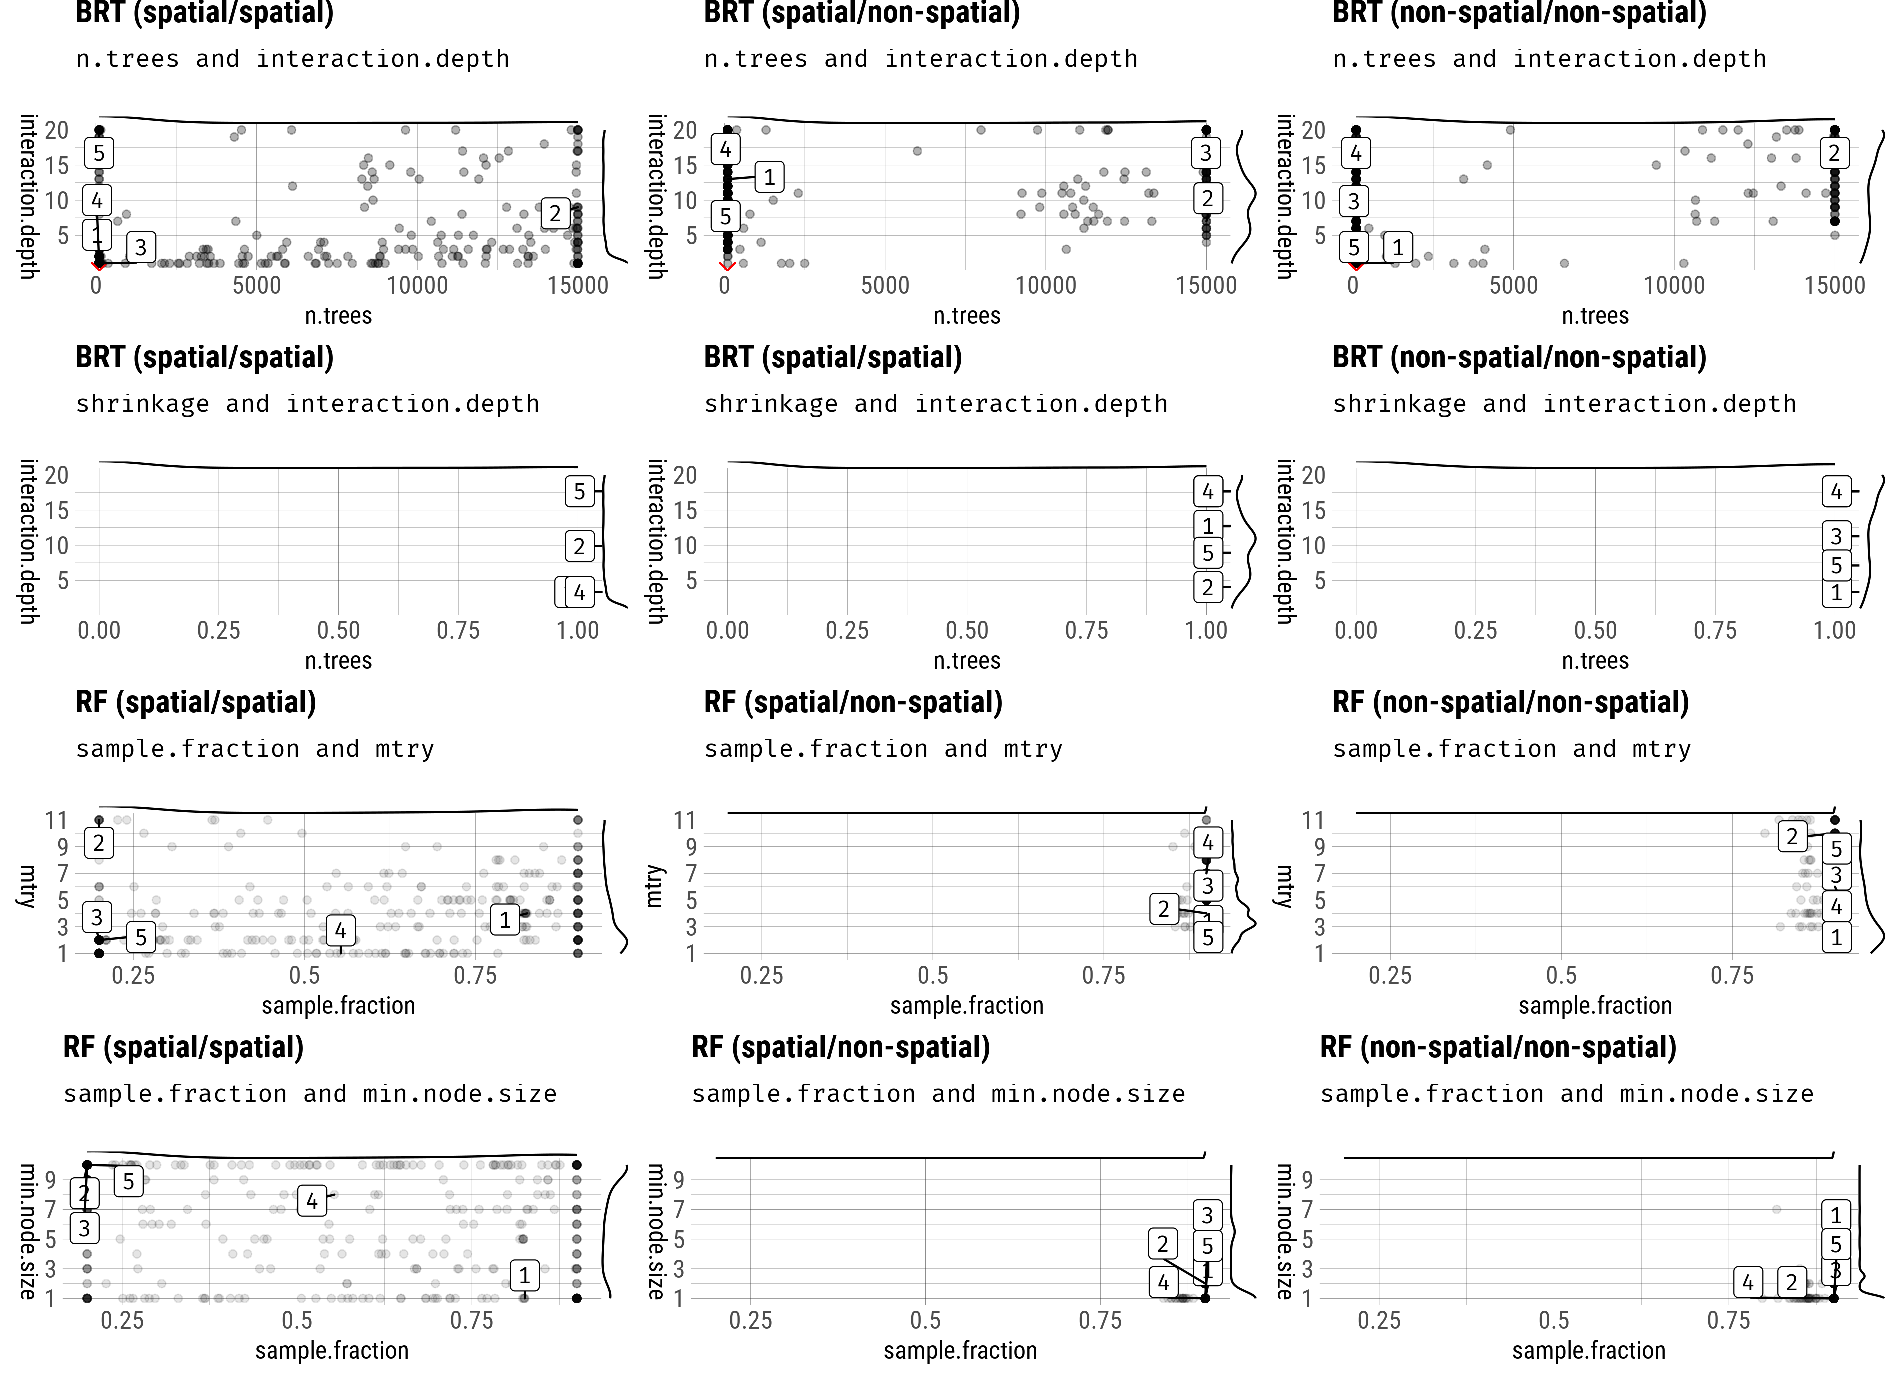
\includegraphics[angle=90, height = 0.55\textheight] {tuning_effects_appendix_mbo.pdf}}
		\caption[]{Best hyperparameter settings by fold (500 total) each estimated from 100 (30/70) SMBO tuning iterations per fold using five-fold cross-validation. Split by spatial and non-spatial partitioning setup and model type.
			Red crosses indicate the default hyperparameters of the respective model.
			Black dots represent the winning hyperparameter setting of each fold.
			The labels ranging from one to five show the winning hyperparameter settings of the first five folds}
		\label{fig:best_parameter_combs_app}
	\end{center}
\end{figure}

\pagebreak

\section{SMBO optimization paths for all models}

\begin{figure} [ht]
	\begin{center}
		\makebox[\textwidth]{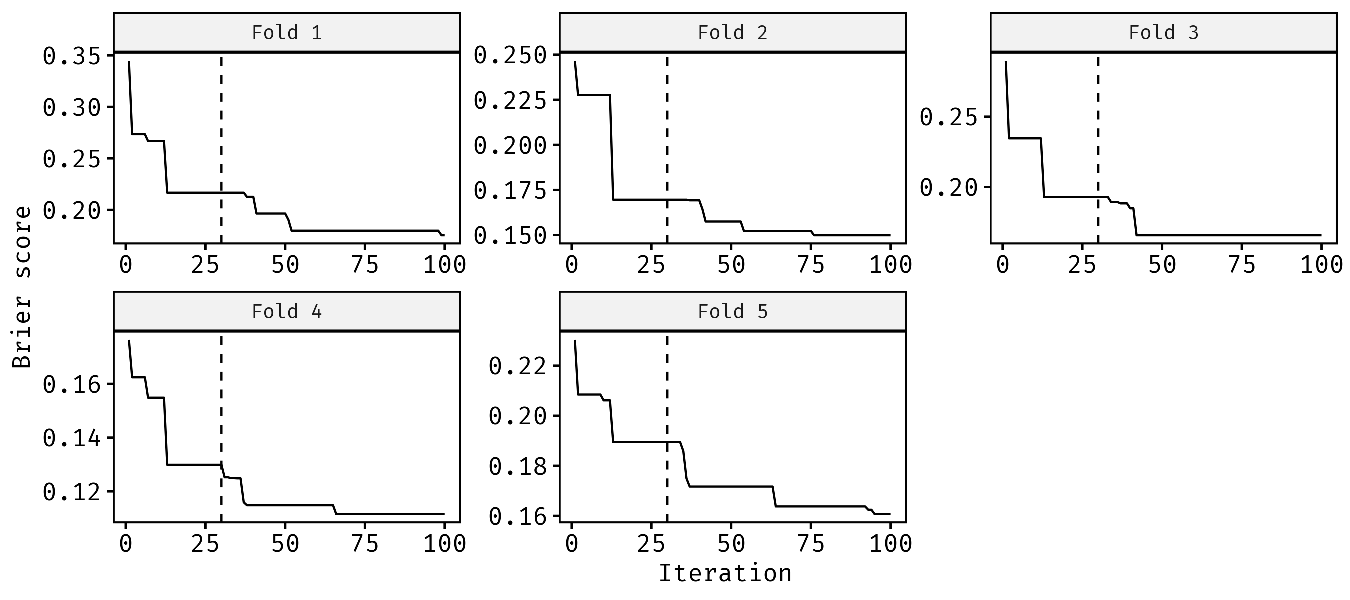
\includegraphics[width=\textwidth] {opt-paths-BRT.pdf}}
		\caption[]{SMBO optimization paths of the first five folds of the \emph{spatial/spatial} for \ac{BRT}. The dashed line marks the border between the initial design (30 randomly composed hyperparameter settings) and the sequential optimization part in which each setting was proposed using information from the prior evaluated settings.}
		\label{fig:optimization_paths_brt}
	\end{center}
\end{figure}

\begin{figure} [ht]
	\begin{center} 
		\makebox[\textwidth]{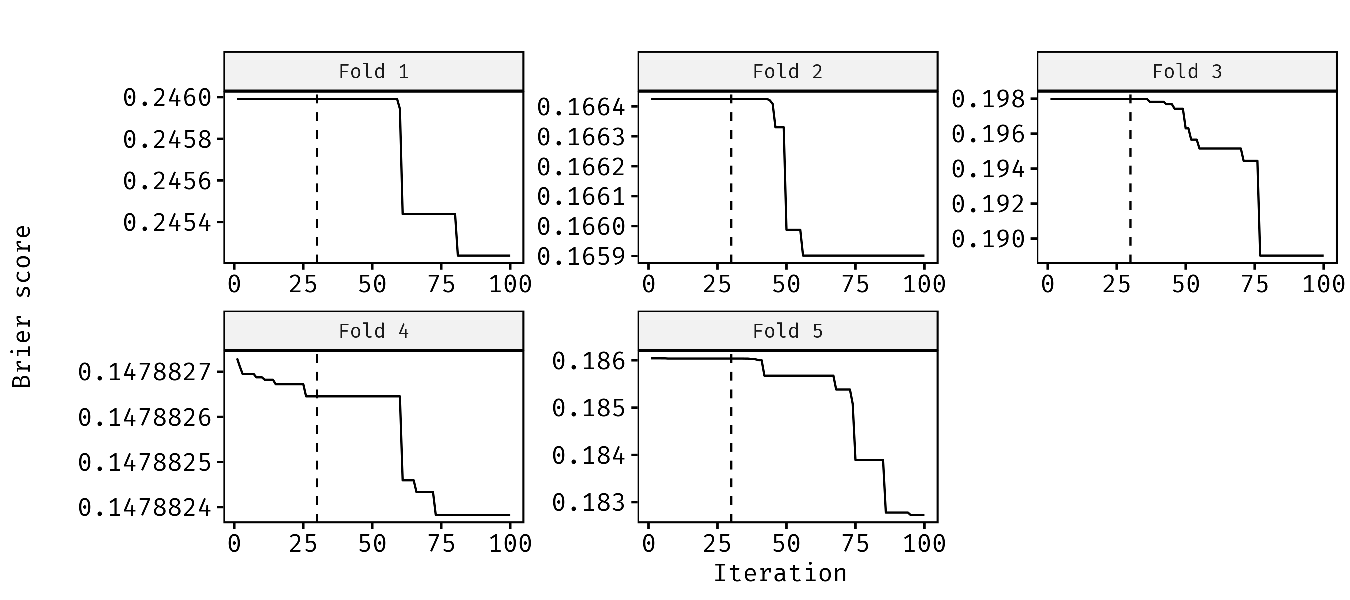
\includegraphics[width=\textwidth] {opt-paths-GAM.pdf}}
		\caption[]{SMBO optimization paths of the first five folds of the \emph{spatial/spatial} for \ac{GAM}. The dashed line marks the border between the initial design (30 randomly composed hyperparameter settings) and the sequential optimization part in which each setting was proposed using information from the prior evaluated settings.}
		\label{fig:optimization_paths_gam}
	\end{center}
\end{figure}

\begin{figure} [ht]
	\begin{center}
		\makebox[\textwidth]{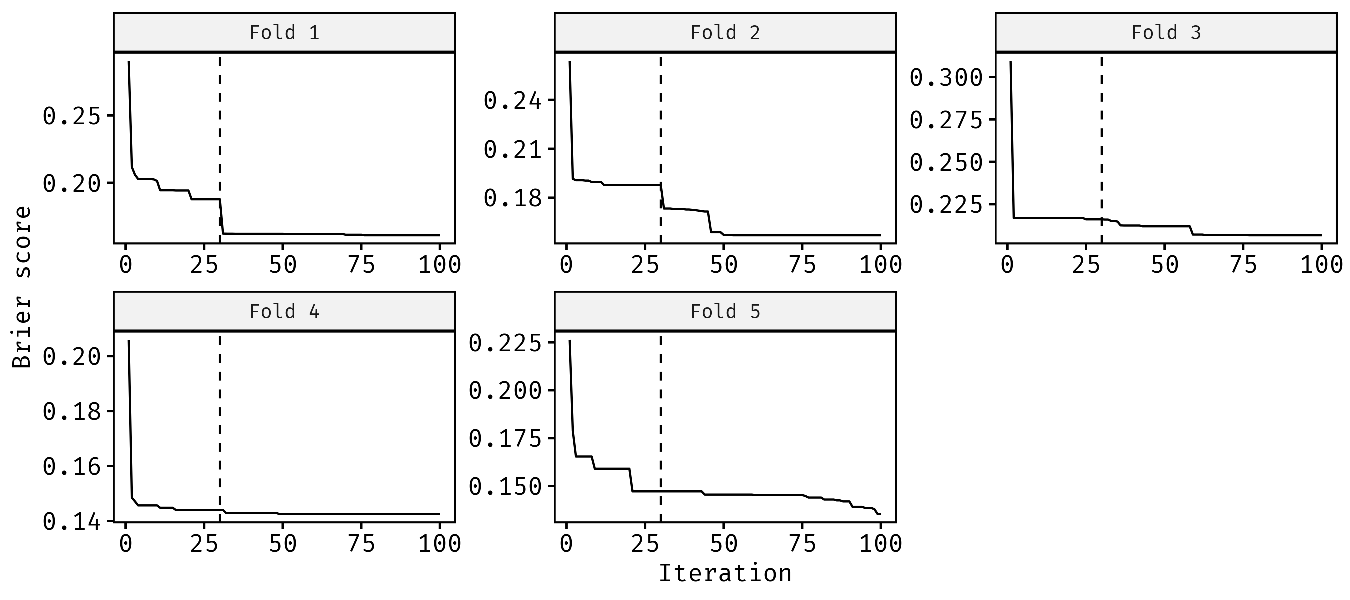
\includegraphics[width=\textwidth] {opt-paths-KNN.pdf}}
		\caption[]{SMBO optimization paths of the first five folds of the \emph{spatial/spatial} for \ac{KNN}. The dashed line marks the border between the initial design (30 randomly composed hyperparameter settings) and the sequential optimization part in which each setting was proposed using information from the prior evaluated settings.}
		\label{fig:optimization_paths_knn}
	\end{center}
\end{figure}

\begin{figure} [ht]
	\begin{center}
		\makebox[\textwidth]{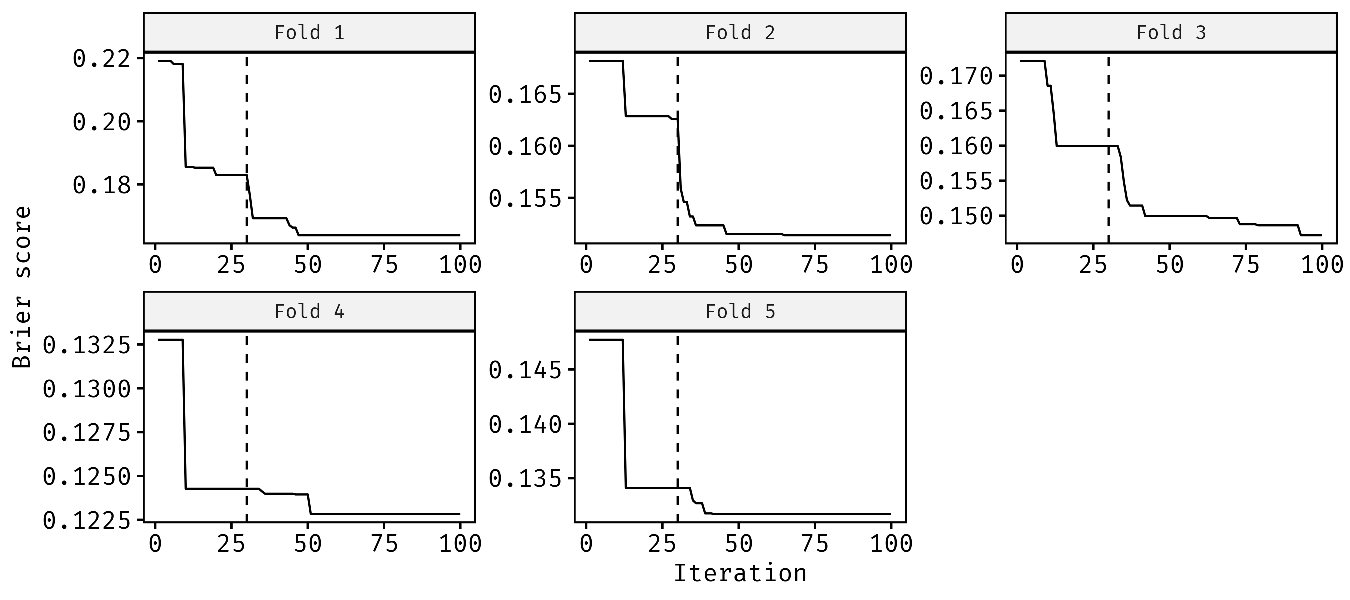
\includegraphics[width=\textwidth] {opt-paths-SVM.pdf}}
		\caption[]{SMBO optimization paths of the first five folds of the \emph{spatial/spatial} for \ac{SVM}. The dashed line marks the border between the initial design (30 randomly composed hyperparameter settings) and the sequential optimization part in which each setting was proposed using information from the prior evaluated settings.}
		\label{fig:optimization_paths_svm}
	\end{center}
\end{figure}

\FloatBarrier

\pagebreak

\section*{References}

\bibliography{Bibliography}

\end{document}
